\chapter{Methodology}
This chapter will outline the methods and techniques used to implement and evaluate the experiments of this thesis. The experiments can be divided into two distinct steps: data generation, where a synthetic dataset is constructed, and the meta training where the model is meta-trained on the synthetic data and then tries to adapt to a set of real-world tasks. Section \ref{image-gen} will cover the image generation process. Section \ref{meta-section} will cover the meta training set up and the training of the neural networks. The following two sections, Sections \ref{software} will outline the software tools used in the experiments.

\section{Data Generation}\label{image-gen}
This section will describe the procedure used to generate synthetic training data from \gls{VBS3}. It will outline how environments and objects are manipulated in the simulator in order to create realistic imagery and how meta-information is extracted from the simulator during generation. Also, this section will list the different adjustable parameters in the data generation setup and how changing these influences the quality and characteristics of the generated data.

\subsection{VBS3}
The tool used for generating image data was the Virtual Battlespace 3 (VBS3) version 18.3.3.8. \gls{VBS3} is a desktop tactical trainer and mission rehearsal software system developed by Bohemia Interactive Simulations. This software is used by many major military organizations, including the U.S. Army and the U.S. Marine. VBS3 has a large library of over 10,000 high-resolution models. This large amount of models makes it useful for generating image data for a variety of semi-realistic military-related tasks, such as generating vehicle images.

The VBS3 software can be controlled through its graphical user interface or via its internal scripting API. %The scripting API uses Bohemia Interactive Simulations own scripting language called \gls{SQF}.


\subsection{Generation Process}
The image generation process is started by initializing the simulation with a fixed setting and a list of vehicles. The setting is chosen from the available library of terrain maps. There are five different standard environments available in VBS3 (see Section \ref{settings}). For the vehicle classification tasks, a list of 2357 vehicle models is used. These classes were extracted by iterating over the list of vehicle models in the VBS3 documentation. These vehicles include everything from large military vehicles like tanks, airplanes, and aircraft carriers to smaller objects like remote controlled cars and drones. 

After a setting is decided the simulator starts iterating over the provided list of vehicle models. For each vehicle, it will take a fixed number of images. Since the task of interest is standard image classification, only a single object at the time is spawned, although the process is easily extended to many objects. After all images of all vehicles have been taken, the simulation will be restarted with a new setting.

The process of generating an image starts by spawning an instance of the current model in a random location in the in-game map. Similarly to ~\textcite{structureddomainrandomization}, the context of the object and setting are taken into account when generating the images. Vehicles that are based in water, like boats, are more likely to be spawned in a body of water. Flying vehicles like drones, planes, and helicopters are either spawned between 2 to 20 meters in the air or spawned laying on the ground. All other land-based vehicles are always spawned standing on the ground in the most realistic way possible. 

After the vehicle has been position in the world, an in-game camera is randomly positioned around the object. The camera is positioned in such a way that the object of interest is clearly visible and not obfuscated completely by the terrain. The distance between the camera and the object is dependent on the size of the objects. For smaller objects like drones, remote-controlled vehicles and smaller boats, the camera is set to be at the most 15 meters from the object. For larger vehicles like transport planes or oil tankers, the camera is given a larger offset, starting from 30 meters to ensure that the object never covers the entire image.

After the in-game camera has found a clear view of the object, the world's lighting and weather effects are randomized, as well as other settings, in order to introduce variance in the images. The camera then takes a photo of the resulting scene, which will be used as training data. Additional meta information, like the current rotation of the object, is also saved. 

After the first photo has been taken, all lighting and weather effects are temporarily disabled in order to create a clearer image. A render mask is then applied to the object, transforming it into a single uniform segment of an easily identified color, such as pink (see Figure. \ref{fig:rendermask}). A second photo is then taken with the same camera as before.

\begin{figure}[H]
\centering
\subcaptionbox{Generated Image}
  {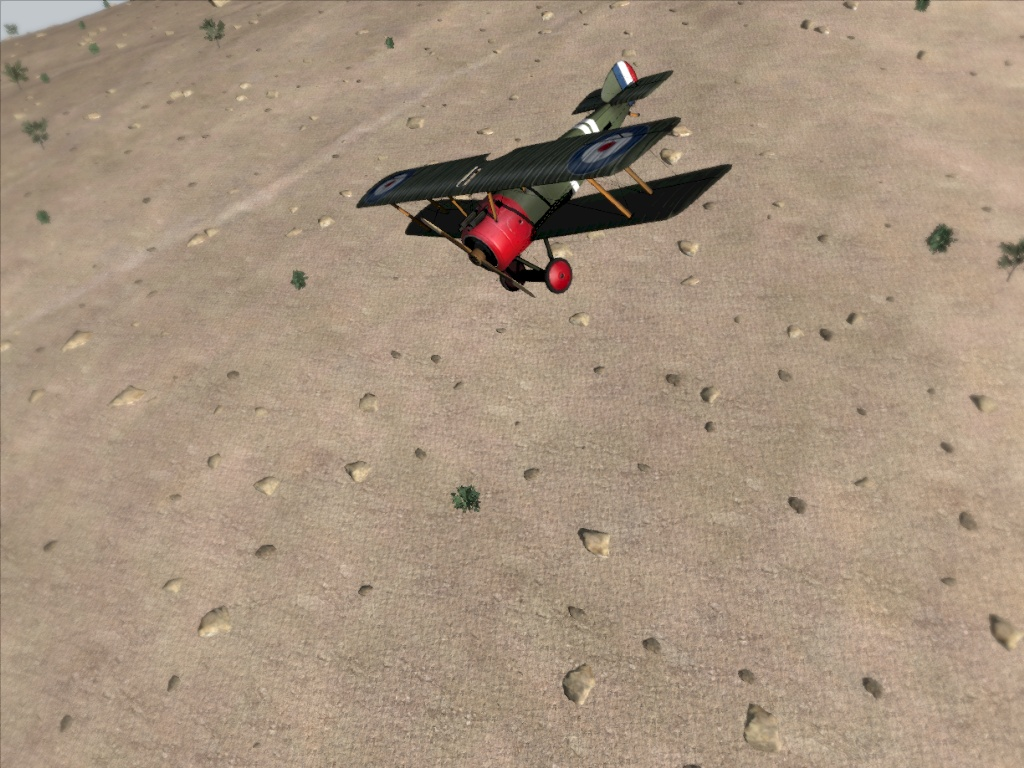
\includegraphics[height=4.4cm]{images/vbs3/bbox/example2.jpg}}
\subcaptionbox{Masked Object}%
  {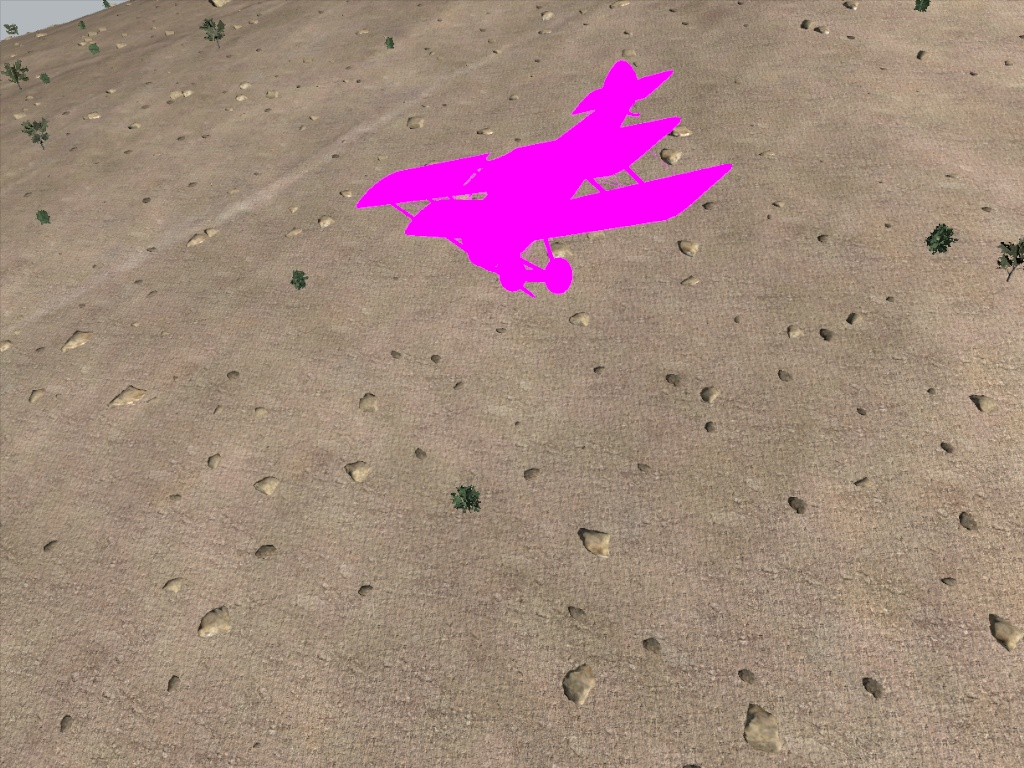
\includegraphics[height=4.4cm]{images/vbs3/bbox/example2-pink.jpg}}
%\subcaptionbox{Extracted Bounding Box}%
%  {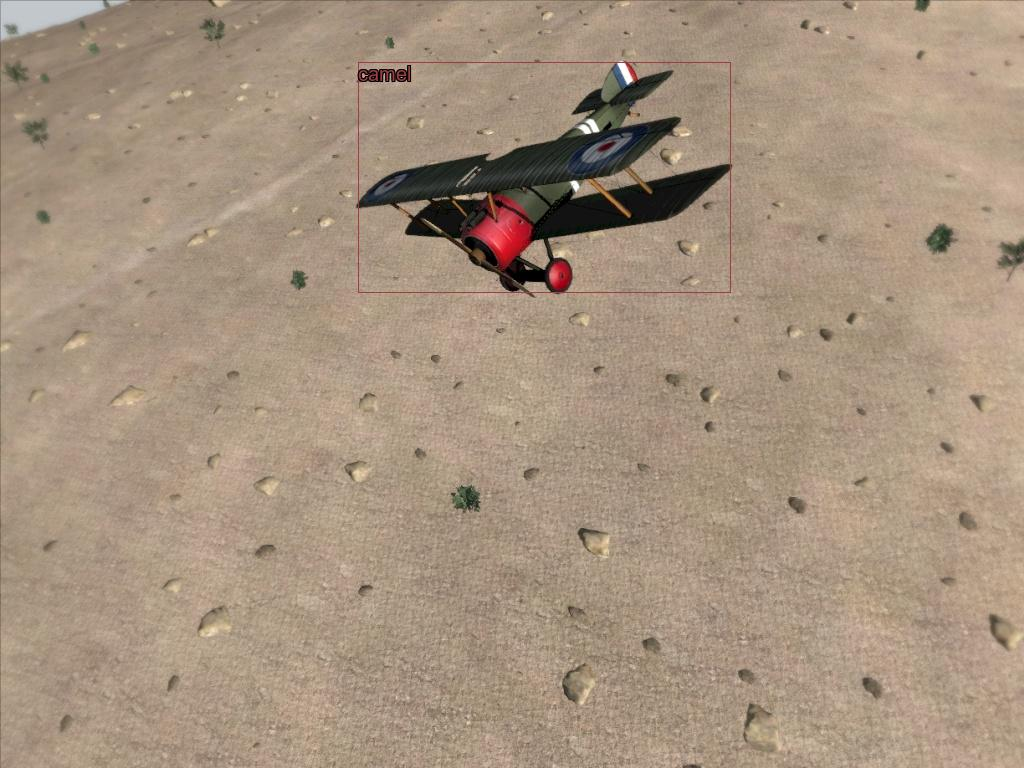
\includegraphics[height=4.4cm]{images/vbs3/bbox/example2-bbox.jpg}}
\caption{}
\label{fig:rendermask}
\end{figure}

Segmentation information and bounding box information is then extracted using the render-masked image. There are several advantages of having access to segmentation information, even if the final target task will not utilize it. It allows for automatic and precise cropping of the object of interest. It also makes it possible to detect bad image samples where the object is hidden or obscured. The simulator, \gls{VBS3}, is not always able to find perfectly suitable camera-angles. Sometimes vegetation and other objects can cover the object. In this thesis, images with an object segment of fewer than 750 pixels were therefore removed in a separate filtering step in order to remove obscured objects. However, this also meant that some of the smaller vehicles had a higher probability of being removed. As a result, some of the classes consisted of fewer images than others.

Between each photo of the same vehicle, the vehicle is moved to a new position within a hundred-meter radius of the previously used position. This range limit is set to allow the simulation to load the background textures properly before the image is taken. If the vehicle is allowed to move over a larger area, the simulation can have a problem loading the background textures with the highest resolution in time, resulting in poor image quality.

This generation process is re-run one time for each of the five available maps, in order to create a high degree of variety in the dataset.

\subsection{Image Randomization}\label{randomization-settings}
The experiments of~\textcite{domainrand},~\textcite{domainrandcars} and~\textcite{structureddomainrandomization} have shown that the variation of the training data can have a substantial effect on the final performance of models trained with synthetic data. Since these methods have never been tested in a meta-learning setting, it is, therefore, essential to determine if the same principles still hold.

In order to investigate this, the simulation setup has been built to allow for certain simulation parameters to be enabled and disabled, which changes how the scenes are randomized. These parameters are: 

\begin{itemize}
    \item \textbf{Context}: Objects are spawned in scenarios that take their real-world context into account (see Figure \ref{with-context}). For example planes and helicopters are spawned in the air, while boats are spawned in bodies of water. Disregarding the context makes the data-generation more akin to standard \gls{DR}, where vehicles can be in any scenario, in any possible position, thus increasing the difficulty of the generated tasks (see Figure \ref{no-context}).
    
    \begin{figure}[H]
    \centering
      {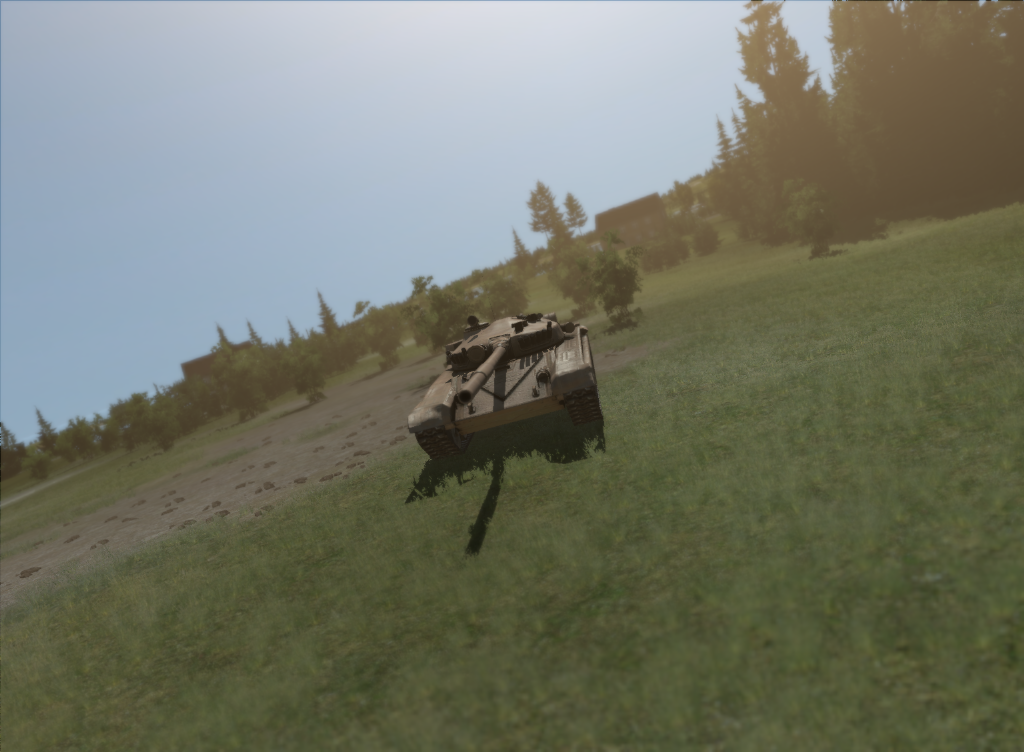
\includegraphics[height=2.4cm, width=3.4cm]{images/vbs3/random-pos/context1}}
      {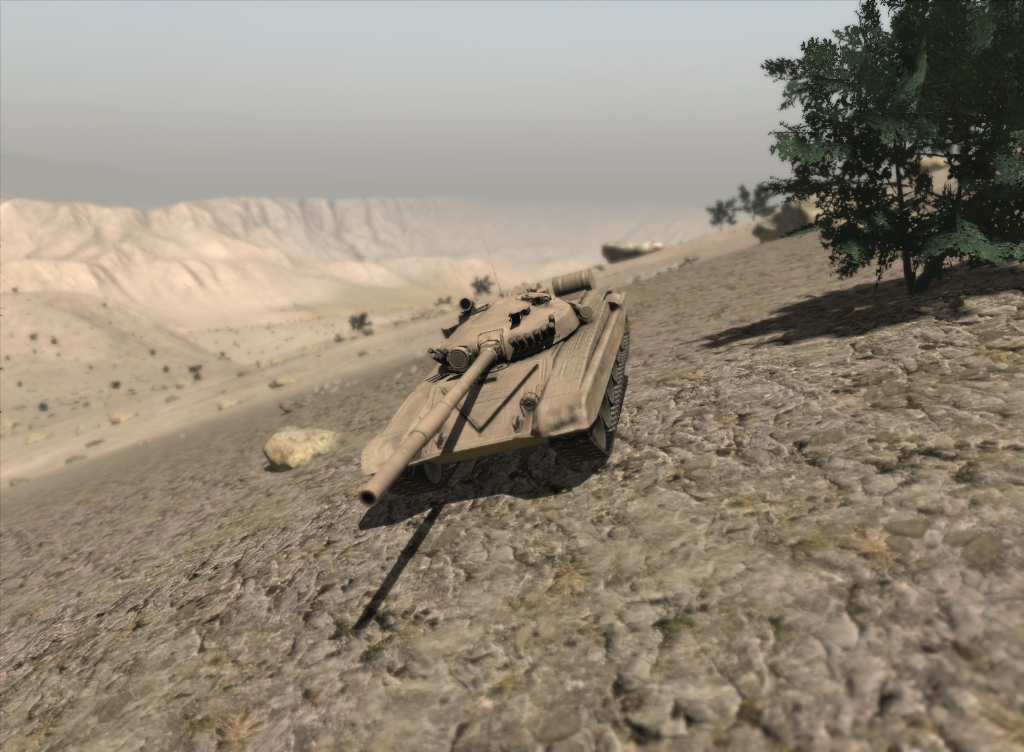
\includegraphics[height=2.4cm, width=3.4cm]{images/vbs3/random-pos/context2}}
      {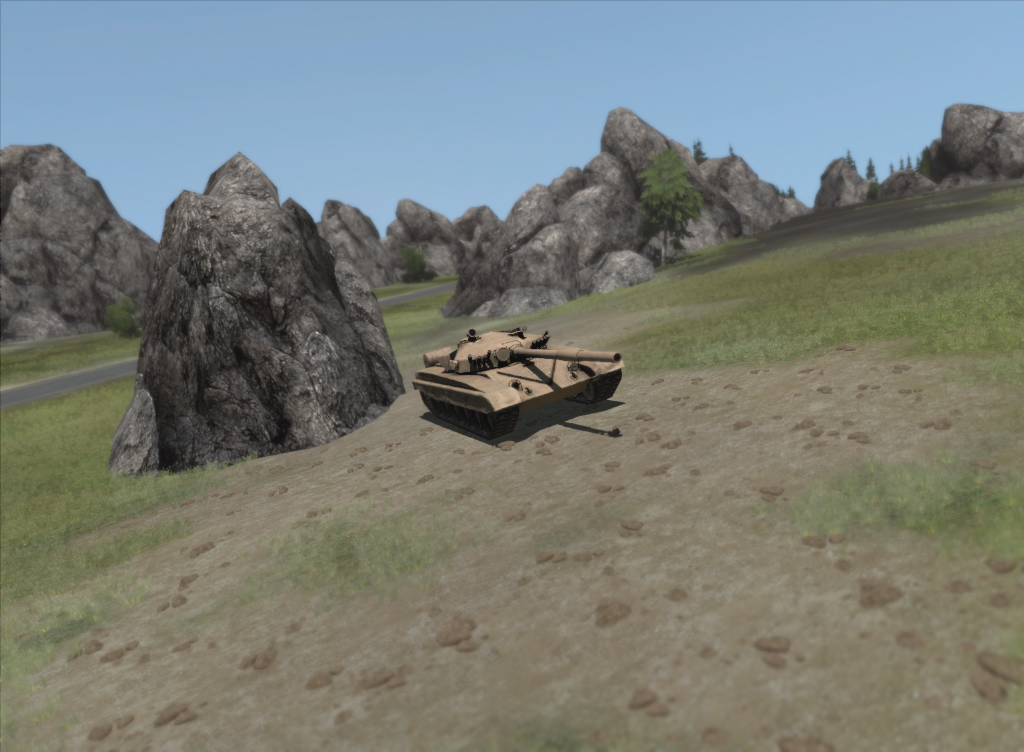
\includegraphics[height=2.4cm, width=3.4cm]{images/vbs3/random-pos/context3}}
    \caption{With context enabled}
    \label{with-context}
    \end{figure}

    \begin{figure}[H]
    \centering
      {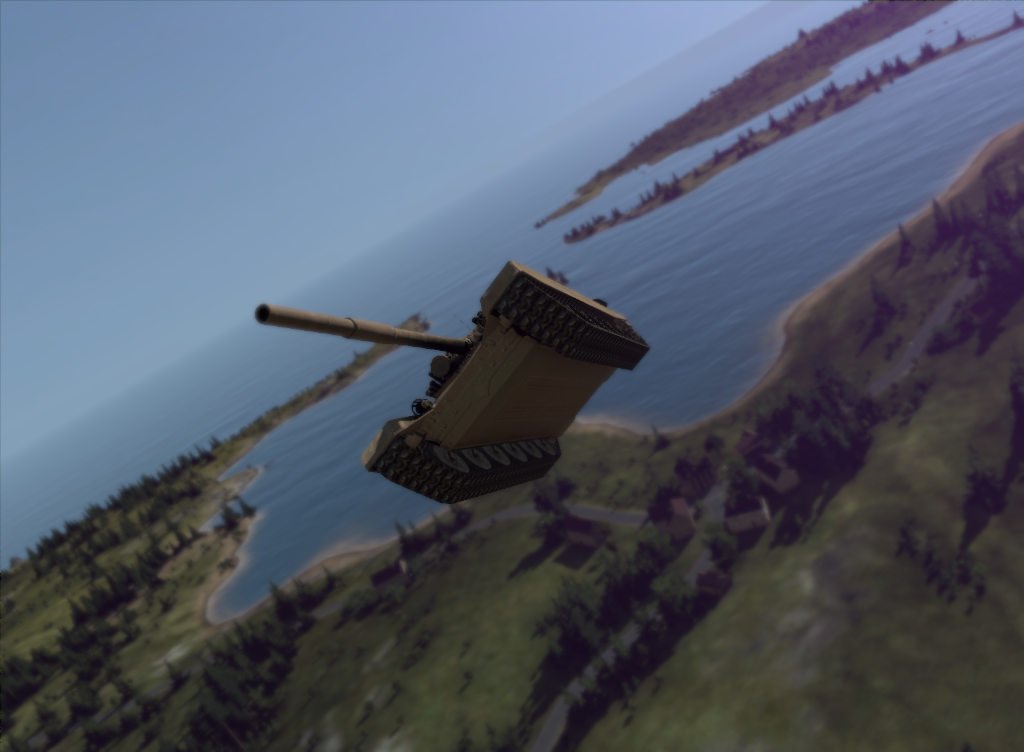
\includegraphics[height=2.4cm, width=3.4cm]{images/vbs3/random-pos/no-context1}}
      {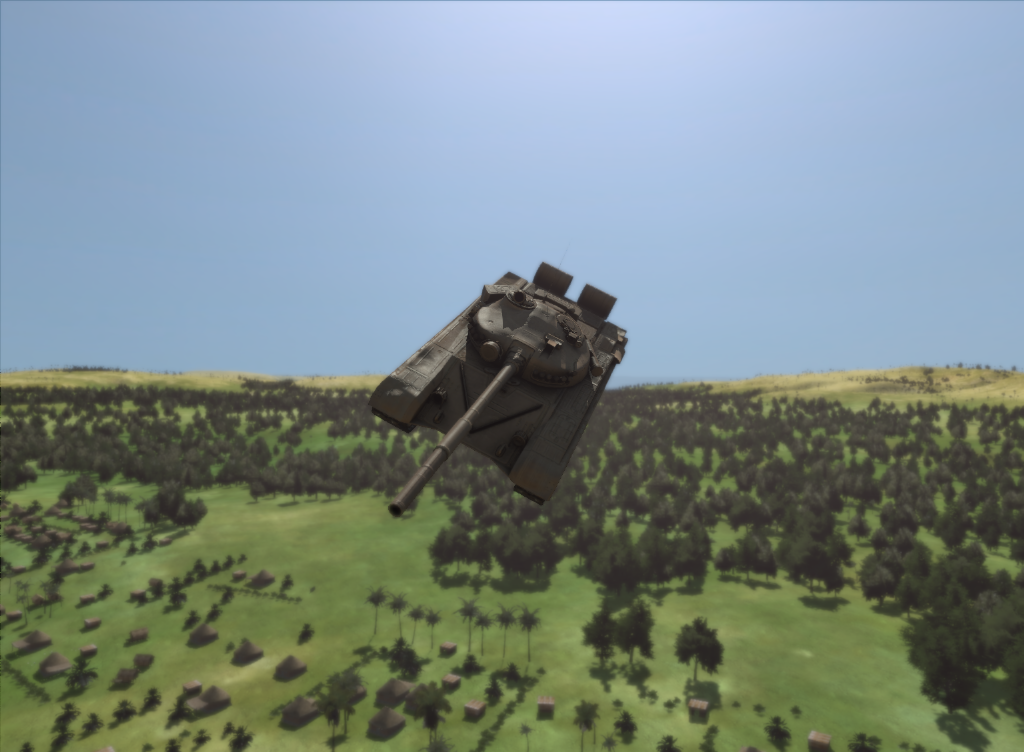
\includegraphics[height=2.4cm, width=3.4cm]{images/vbs3/random-pos/no-context2}}
      {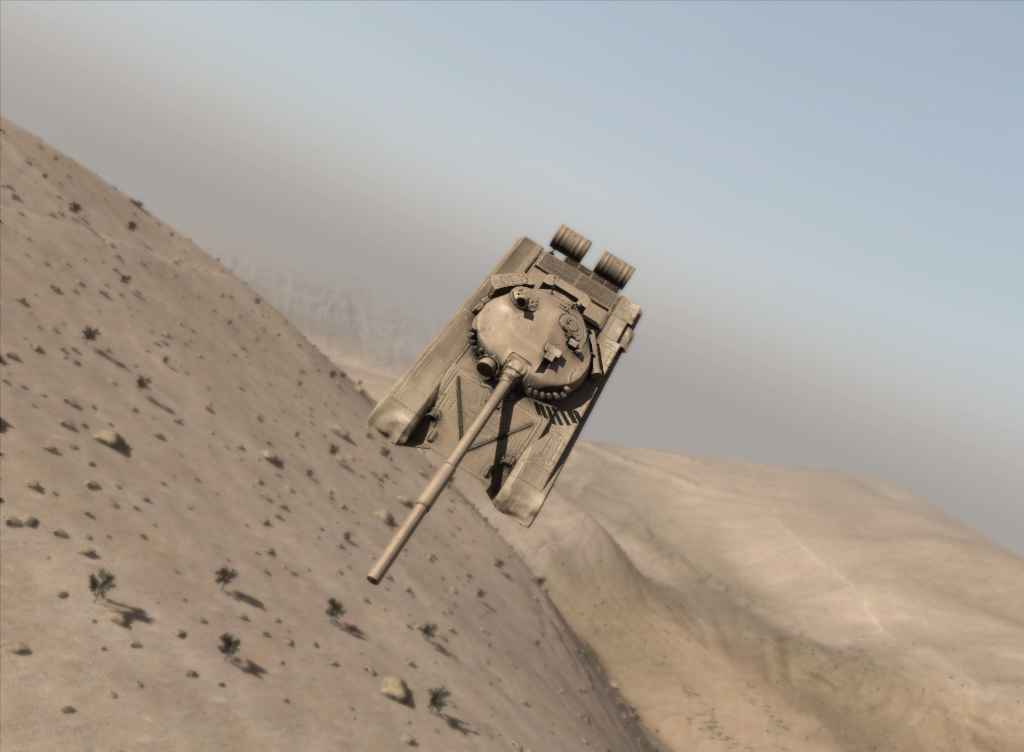
\includegraphics[height=2.4cm, width=3.4cm]{images/vbs3/random-pos/no-context3}}
    \caption{With context disabled}
    \label{no-context}
    \end{figure}

    \item \textbf{Color Scheme/Texture Randomization}: For a subset of the vehicles (around 800), a randomized color is applied to each editable part of the vehicle. Randomizing the textures is a similar approach to what is done both by~\textcite{domainrandcars, structureddomainrandomization}.
    
    \begin{figure}[H]
    \centering
      {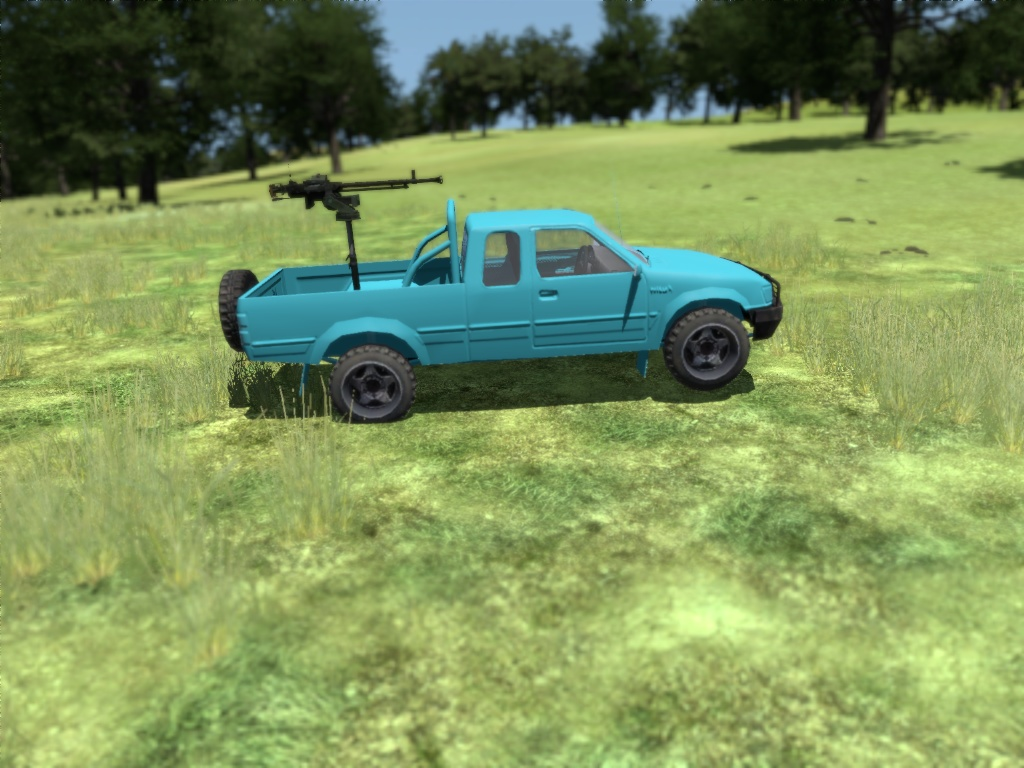
\includegraphics[height=2.4cm, width=3.4cm]{images/vbs3/color-scheme/car/example4-1.jpg}}
      {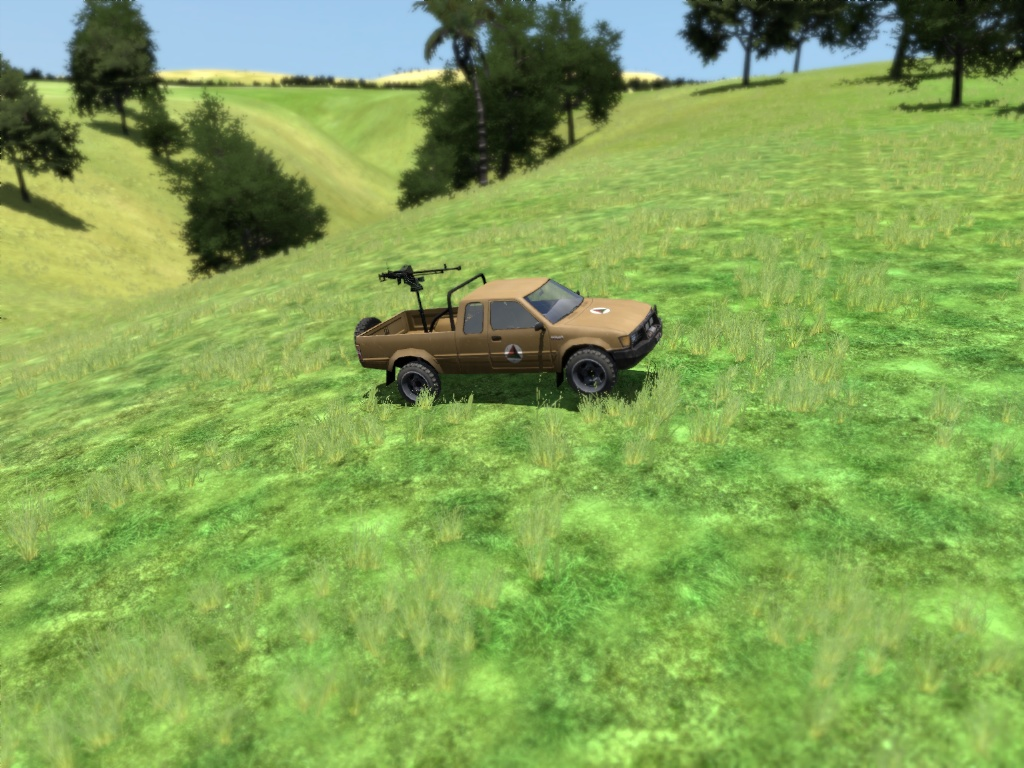
\includegraphics[height=2.4cm, width=3.4cm]{images/vbs3/color-scheme/car/example4-2.jpg}}
      {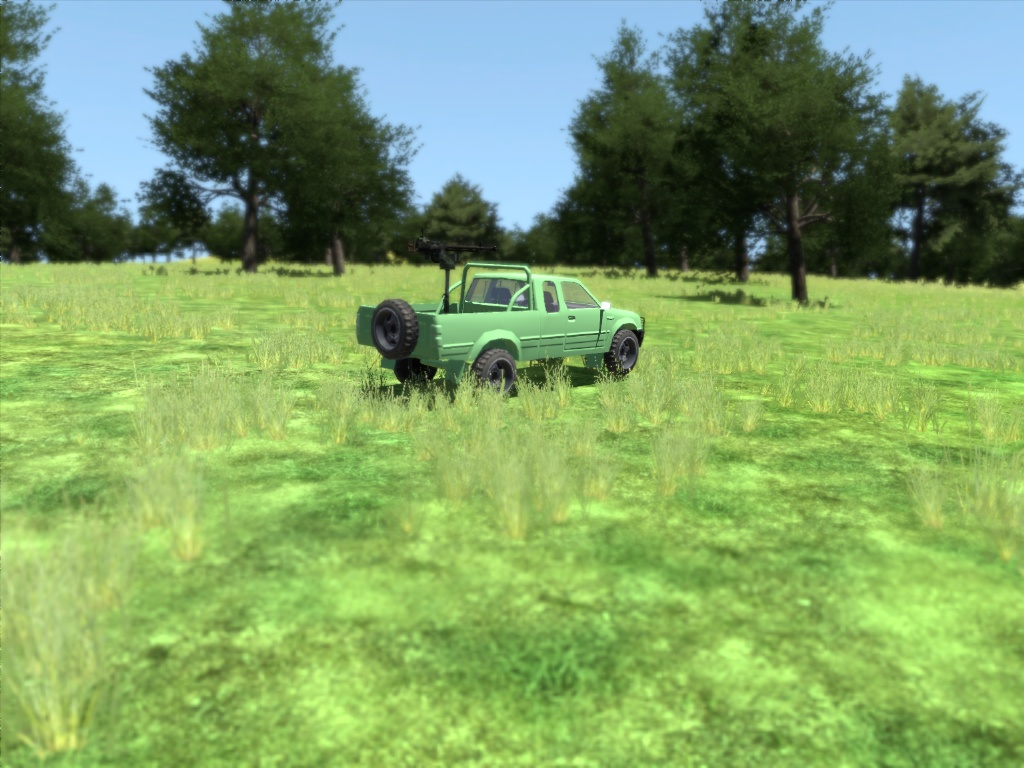
\includegraphics[height=2.4cm, width=3.4cm]{images/vbs3/color-scheme/car/example4-3.jpg}}
      
      {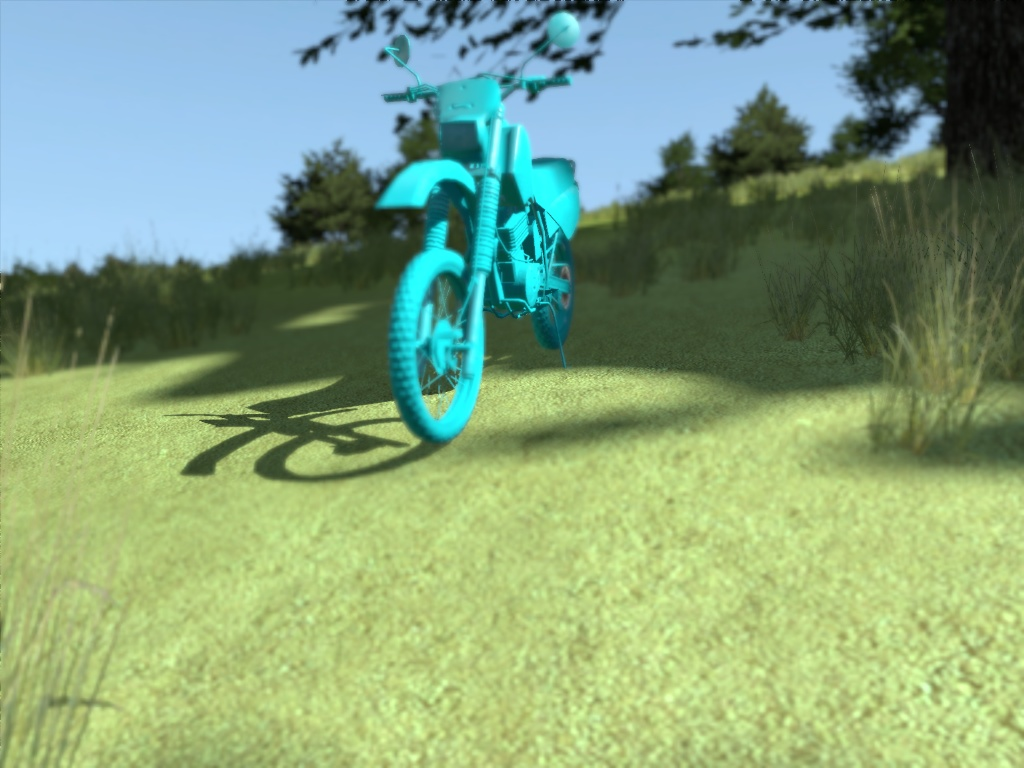
\includegraphics[height=2.4cm, width=3.4cm]{images/vbs3/color-scheme/bike/example4-4.jpg}}
      {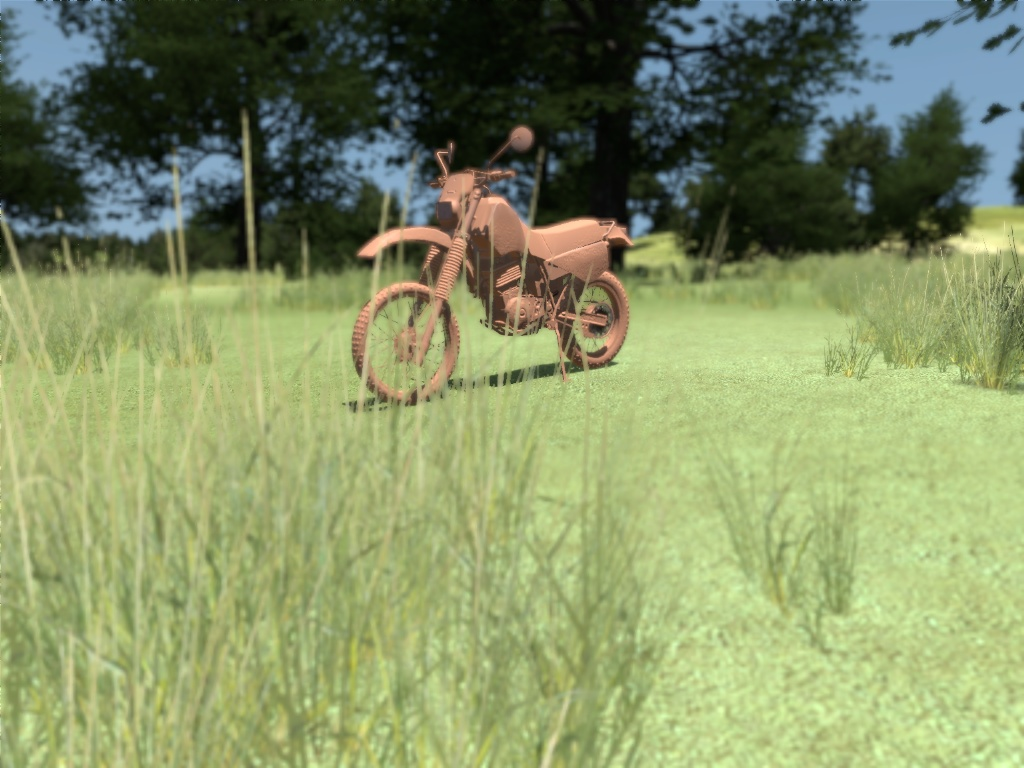
\includegraphics[height=2.4cm, width=3.4cm]{images/vbs3/color-scheme/bike/example4-5.jpg}}
      {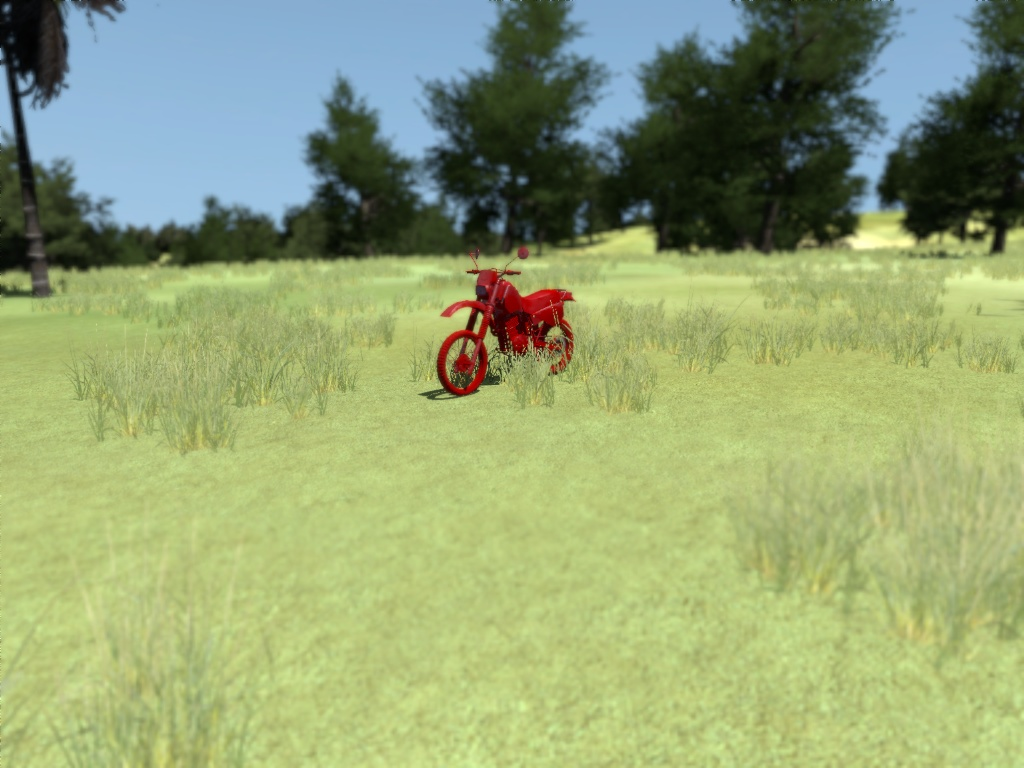
\includegraphics[height=2.4cm, width=3.4cm]{images/vbs3/color-scheme/bike/example4-6.jpg}}
      
        {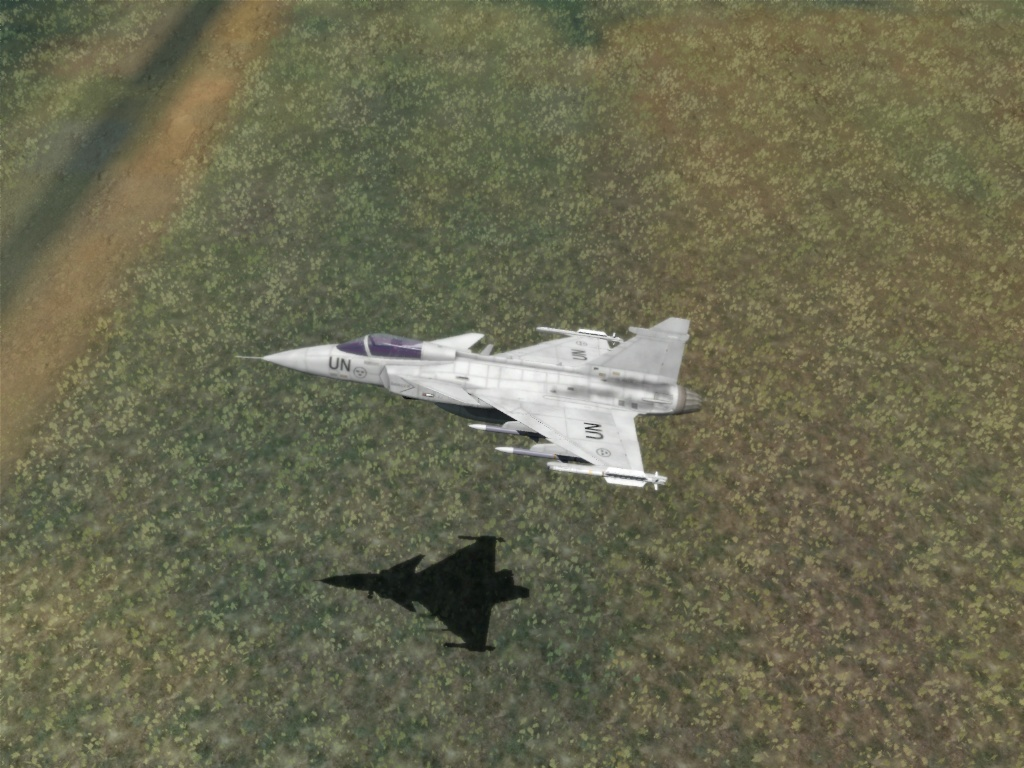
\includegraphics[height=2.4cm, width=3.4cm]{images/vbs3/color-scheme/plane/example4-7.jpg}}
      {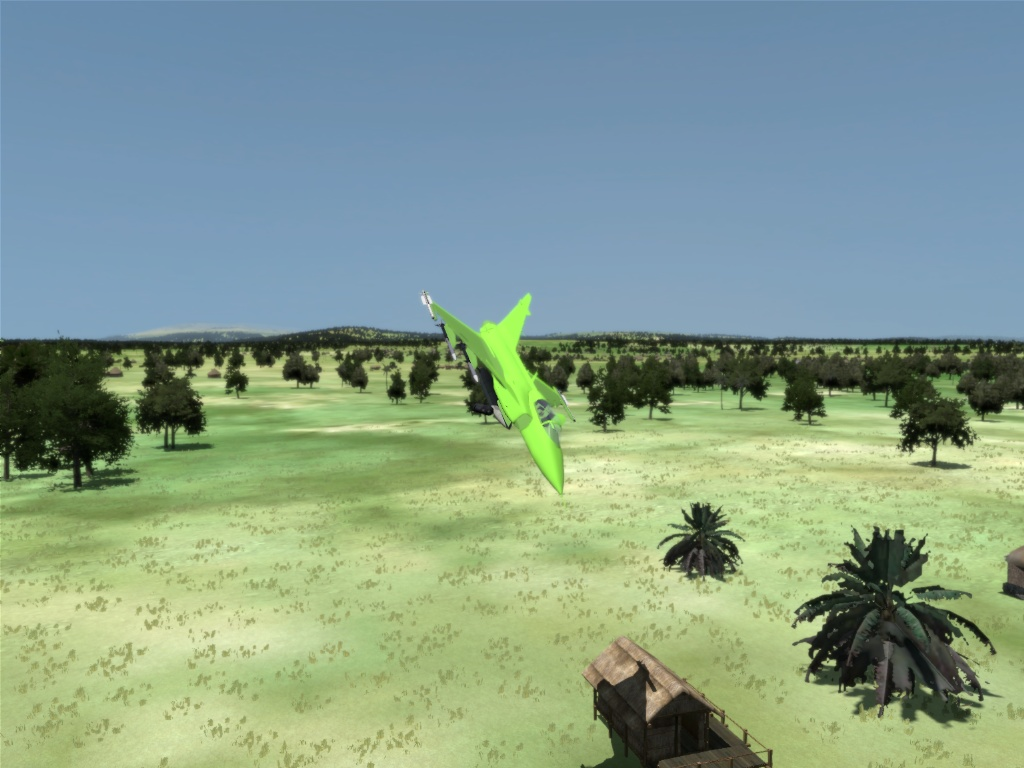
\includegraphics[height=2.4cm, width=3.4cm]{images/vbs3/color-scheme/plane/example4-8.jpg}}
      {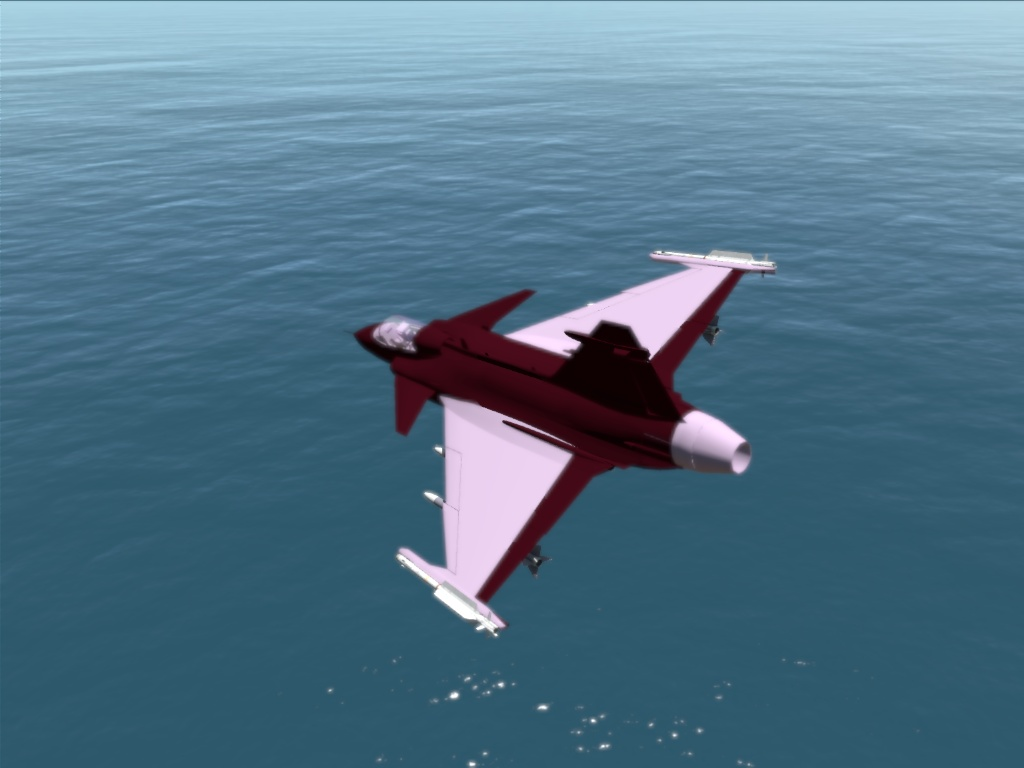
\includegraphics[height=2.4cm, width=3.4cm]{images/vbs3/color-scheme/plane/example4-9.jpg}}
    \caption{Different vehicle models with different color scheme}
    \label{color-scheme}
    \end{figure}
    
    \item \textbf{Lighting}:~\textcite{domainrandcars} showed that variations in lighting could have a huge effect on performance. Outlined here are the different methods for randomizing lighting in the simulation. Examples of their combined effect can be seen in Figure \ref{lighting-example}.

    \begin{itemize}
        \item \textbf{Time}: The time of the day is randomly chosen between the range of hours in which the sun is still visible. Changing the internal time results in the sun, the main lighting source, being in various positions, resulting in both different degrees of lighting intensity as well as different shadow shapes (see Figure \ref{rand-time}). 
        \begin{figure}[H]
        \centering
        \subcaptionbox{}
          {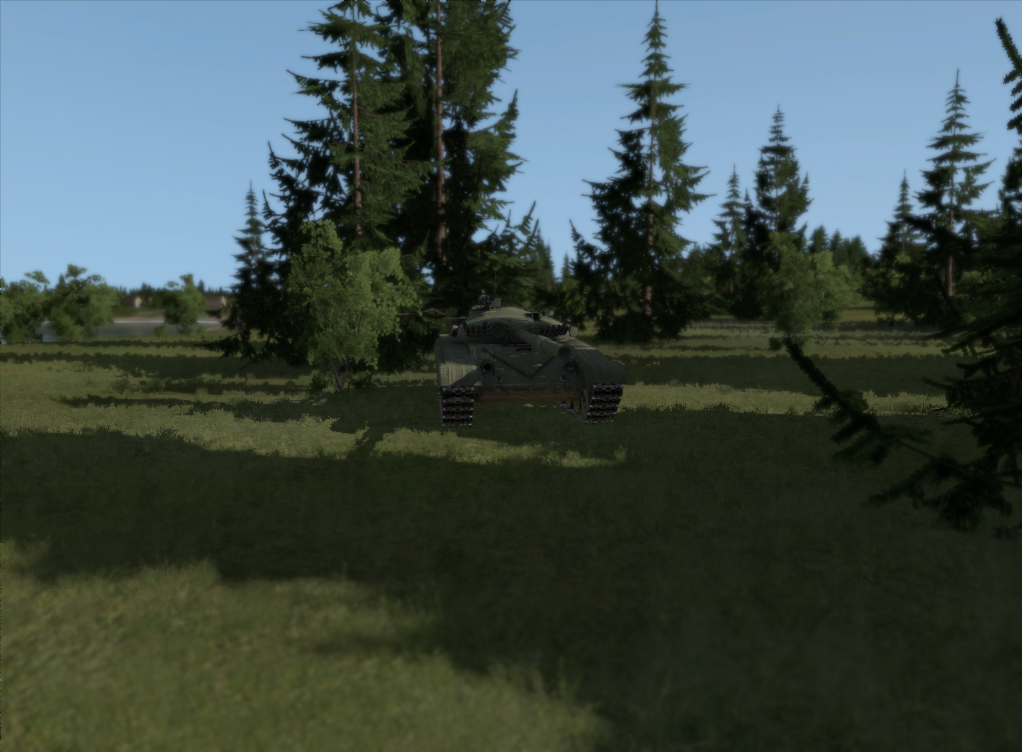
\includegraphics[height=2.4cm, width=3.4cm]{images/vbs3/random-light/time/time-0.png}}
        \subcaptionbox{}%
          {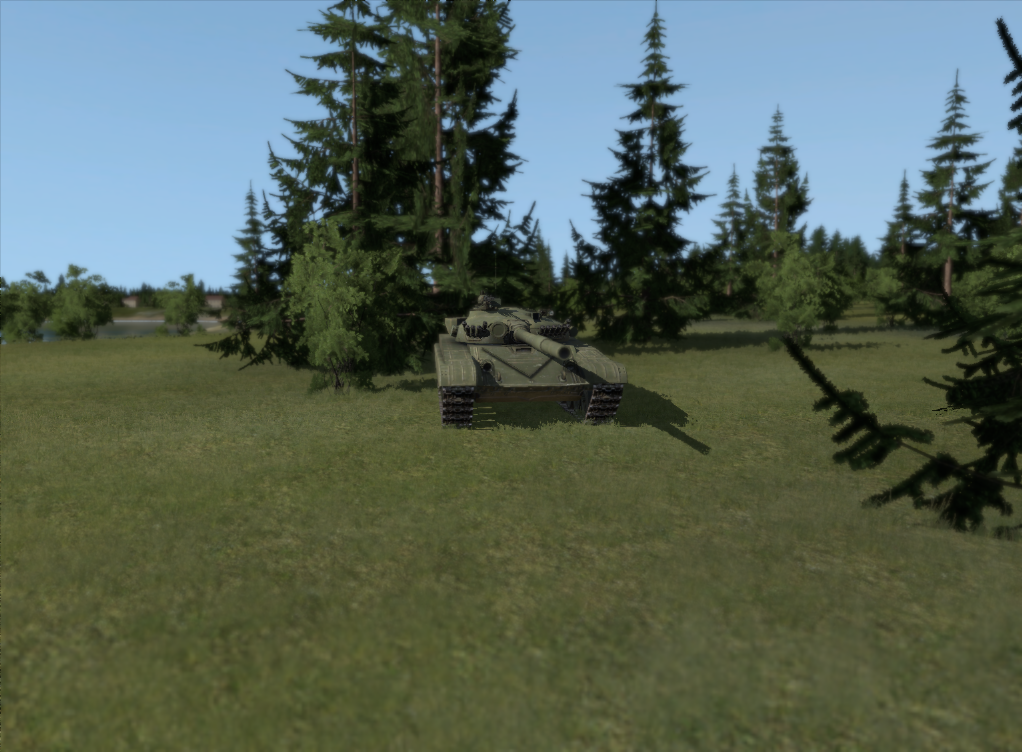
\includegraphics[height=2.4cm, width=3.4cm]{images/vbs3/random-light/time/time-3.png}}
        \subcaptionbox{}%
          {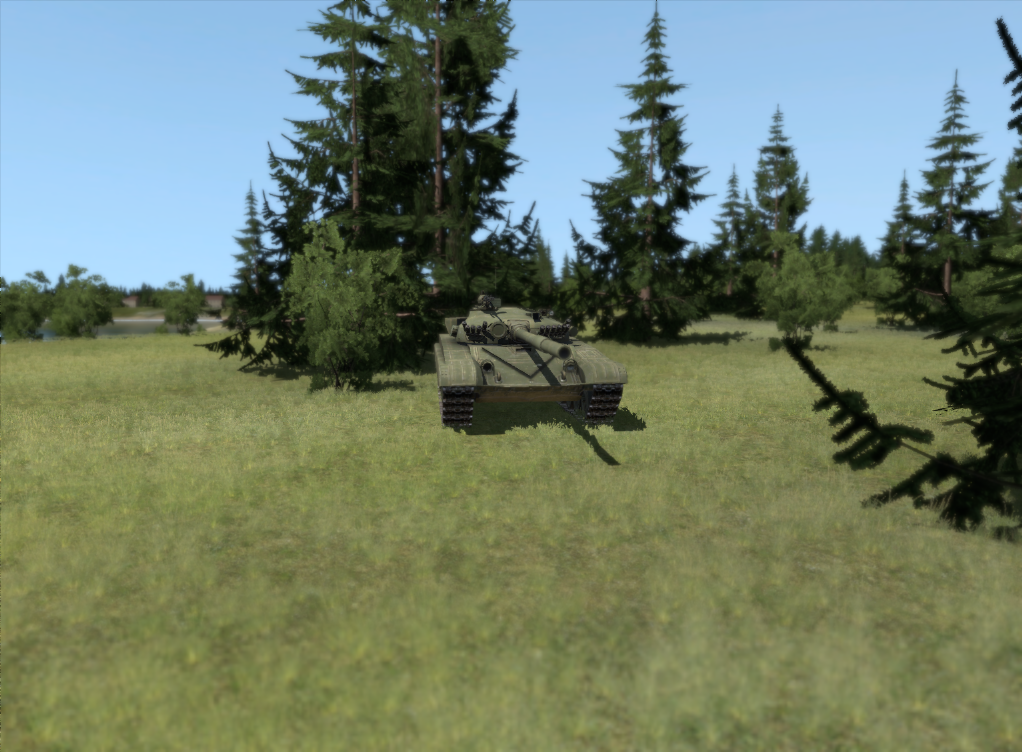
\includegraphics[height=2.4cm, width=3.4cm]{images/vbs3/random-light/time/time-5.png}}
        \caption{Randomized Time}
                \label{rand-time}
        \end{figure}
    
        \item \textbf{Crepuscular Rays}: This setting adjusts the color of light rays coming from the in-game sun, as well as the transparency of these rays. Randomizing this configuration results in a high degree of color variation in the images, but can also make the images blurrier (see Figure \ref{rand-rays}). 
     
        \begin{figure}[H]
        \centering
        \subcaptionbox{}
          {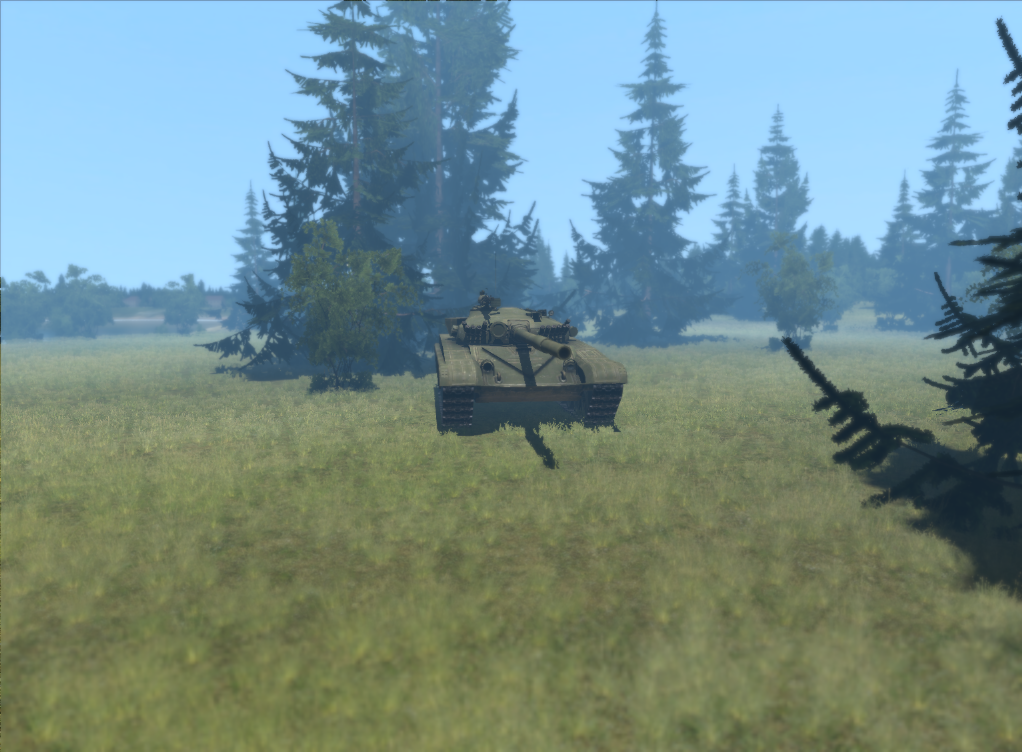
\includegraphics[height=2.4cm, width=3.4cm]{images/vbs3/random-light/ray/rays-0.png}}
        \subcaptionbox{}%
          {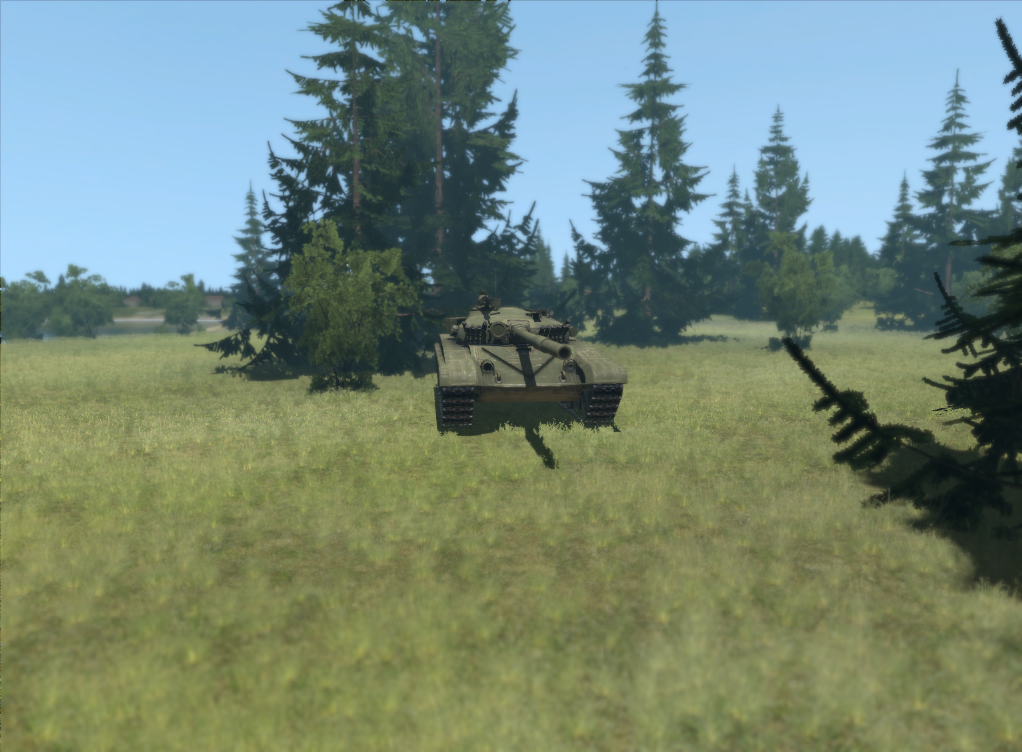
\includegraphics[height=2.4cm, width=3.4cm]{images/vbs3/random-light/ray/rays-1.png}}
        \subcaptionbox{}%
          {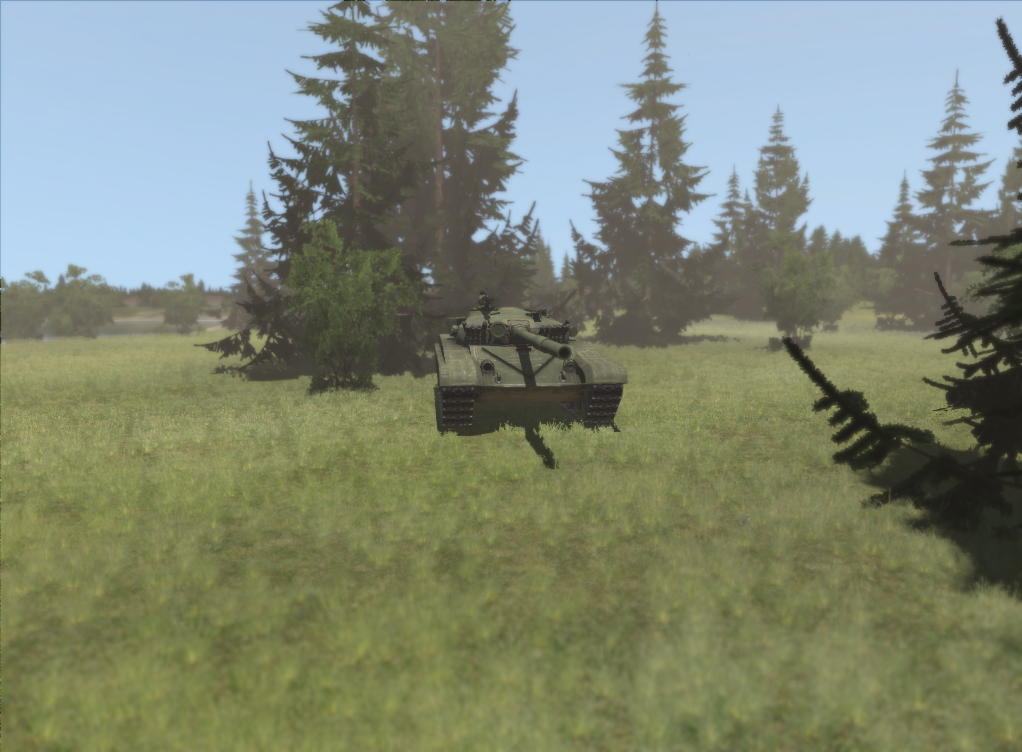
\includegraphics[height=2.4cm, width=3.4cm]{images/vbs3/random-light/ray/rays-4.png}}

        \caption{Randomized Ray Color using VBS3's God Rays}
                \label{rand-rays}
        \end{figure}
     
        \item \textbf{Weather}: With a given probability random weather configurations are chosen. The weather is configured using three variables, level of rain, level of fog, and level of overcast (see Figure \ref{rand-weather}).
 
        \begin{figure}[H]
        \centering
        \subcaptionbox{}
          {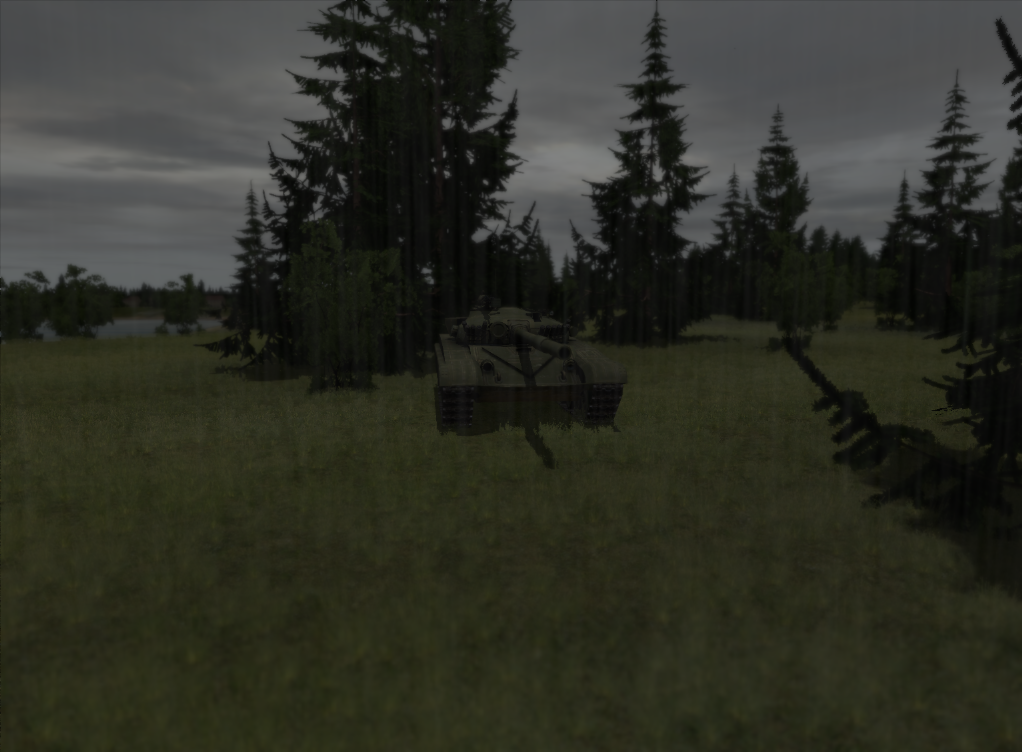
\includegraphics[height=2.4cm, width=3.4cm]{images/vbs3/random-light/weather/weather-0.png}}
        \subcaptionbox{}%
          {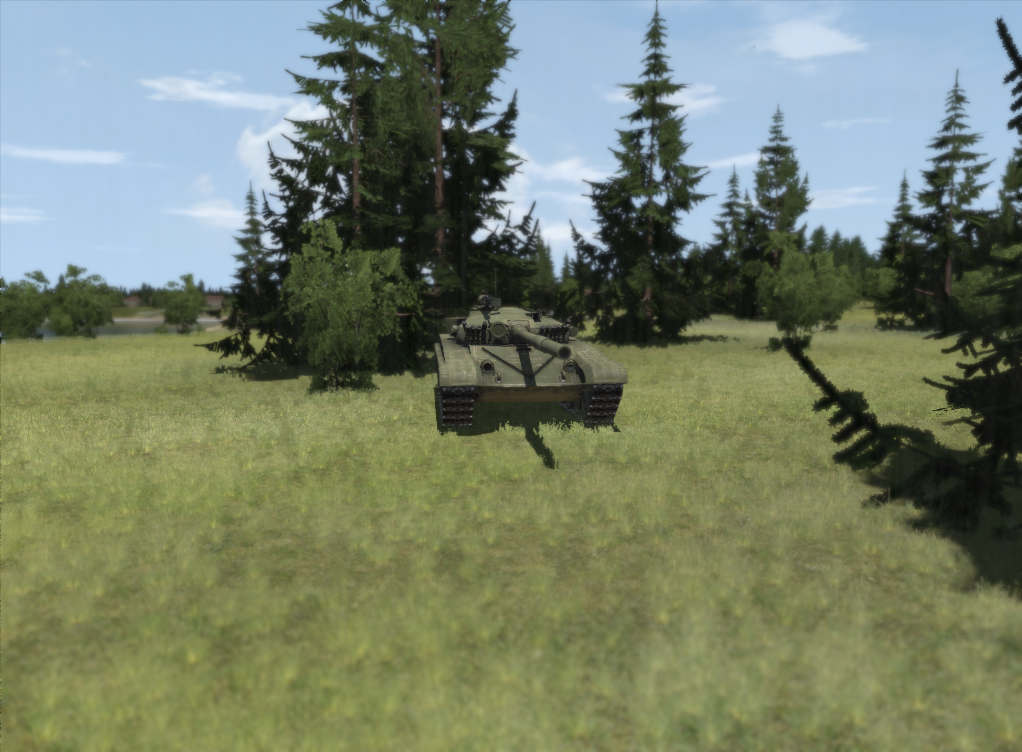
\includegraphics[height=2.4cm, width=3.4cm]{images/vbs3/random-light/weather/weather-1.png}}
        \subcaptionbox{}%
          {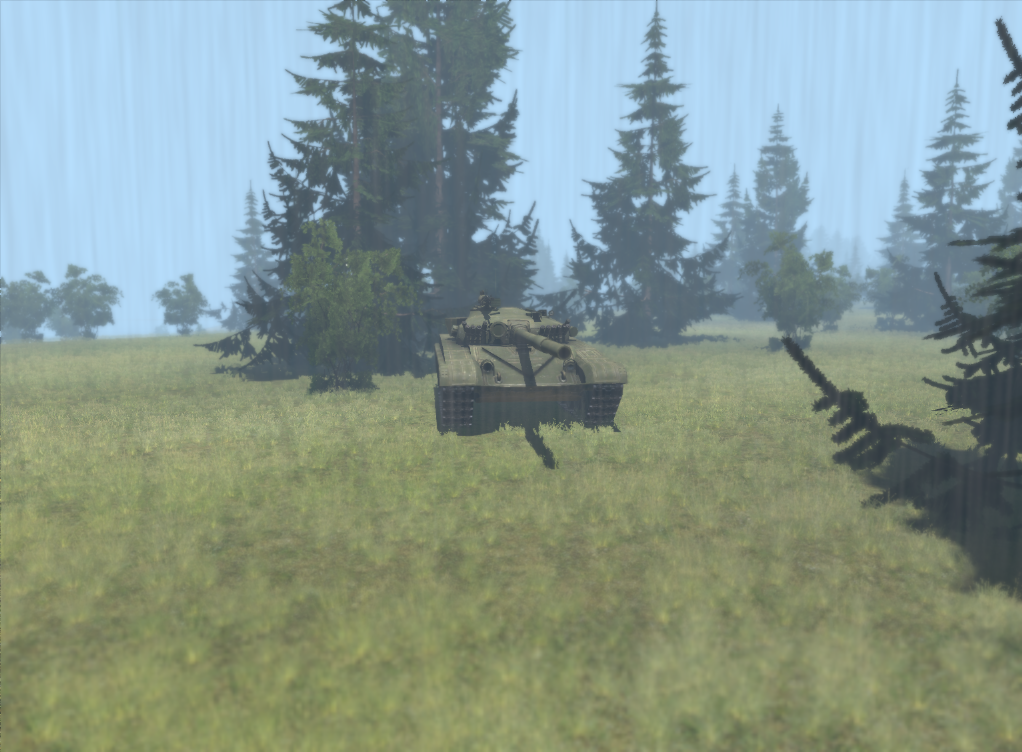
\includegraphics[height=2.4cm, width=3.4cm]{images/vbs3/random-light/weather/weather-3.png}}
        \caption{Randomized Weather}
                \label{rand-weather}
        \end{figure}
             
    \end{itemize}

\end{itemize}


\begin{figure}[H]
\centering
\subcaptionbox{}
  {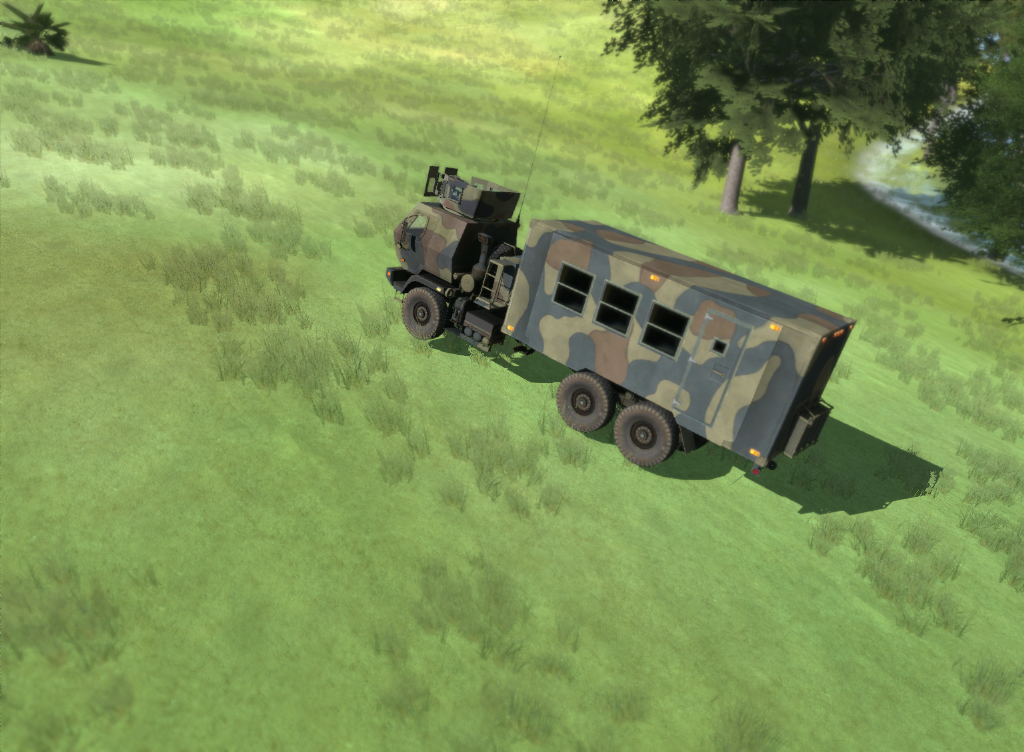
\includegraphics[height=2.4cm, width=3.4cm]{images/vbs3/realistic-lighting/light-variation/1.png}}
\subcaptionbox{}%
  {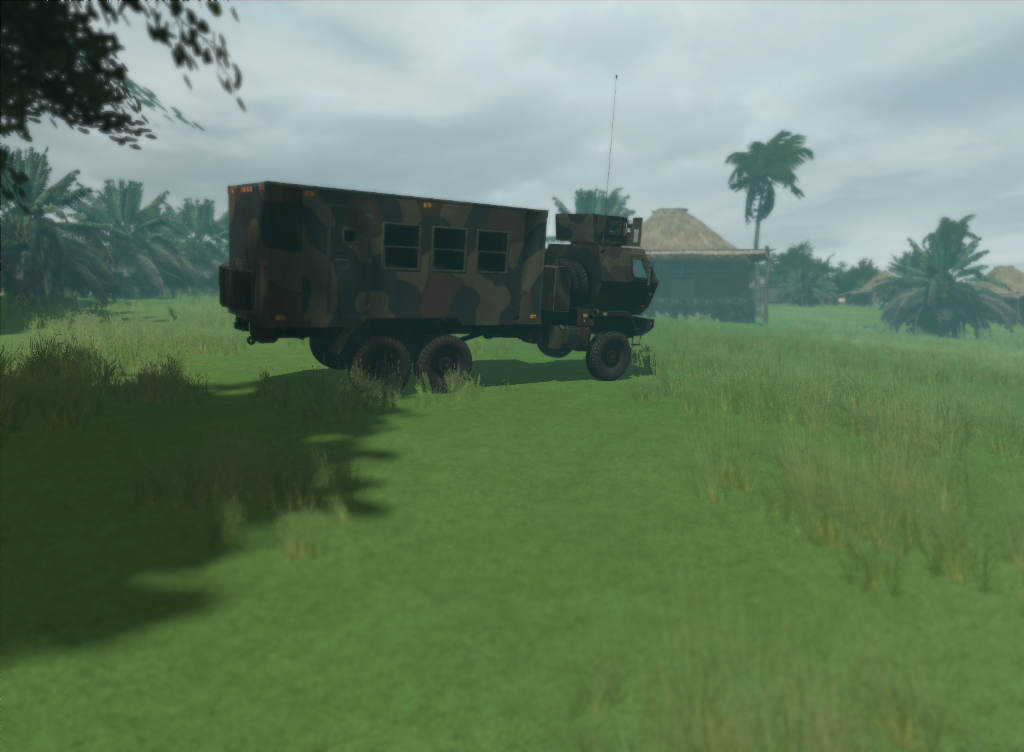
\includegraphics[height=2.4cm, width=3.4cm]{images/vbs3/realistic-lighting/light-variation/2.png}}
\subcaptionbox{}%
  {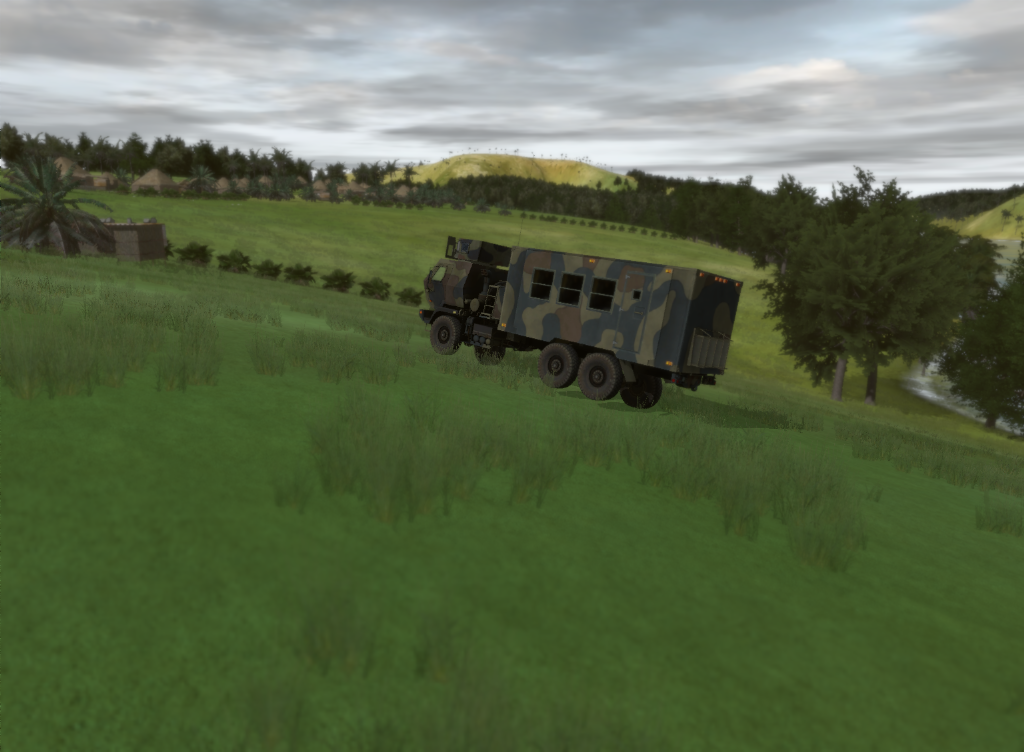
\includegraphics[height=2.4cm, width=3.4cm]{images/vbs3/realistic-lighting/light-variation/3.png}}
\subcaptionbox{}
    {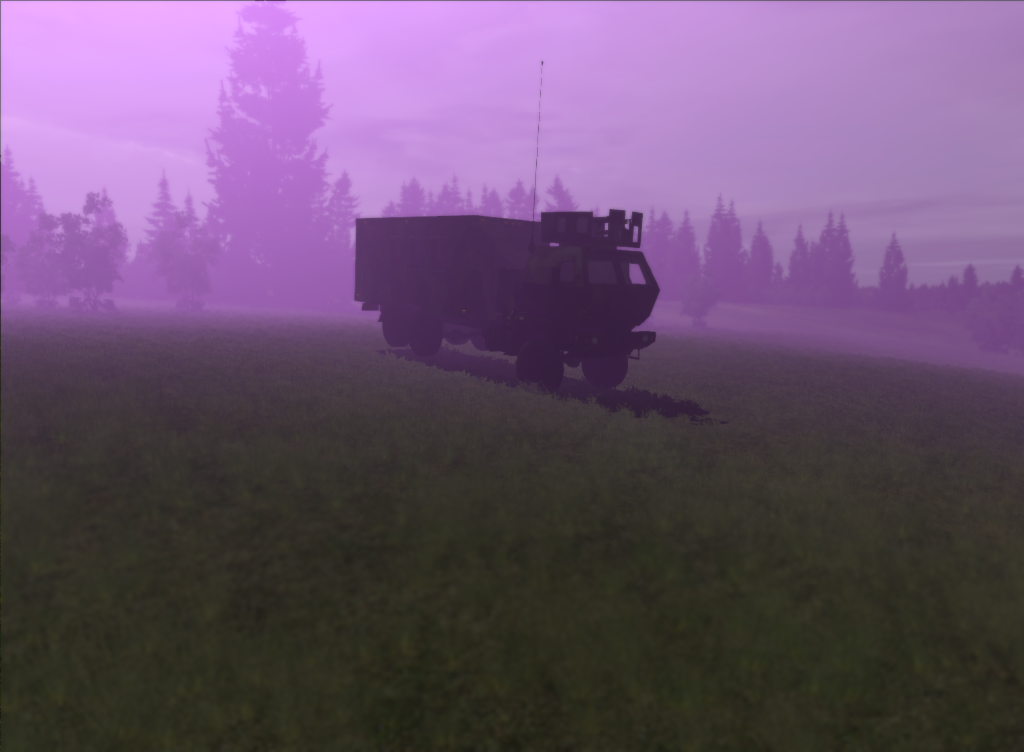
\includegraphics[height=2.4cm, width=3.4cm]{images/vbs3/realistic-lighting/light-variation/8.png}}
\subcaptionbox{}%
  {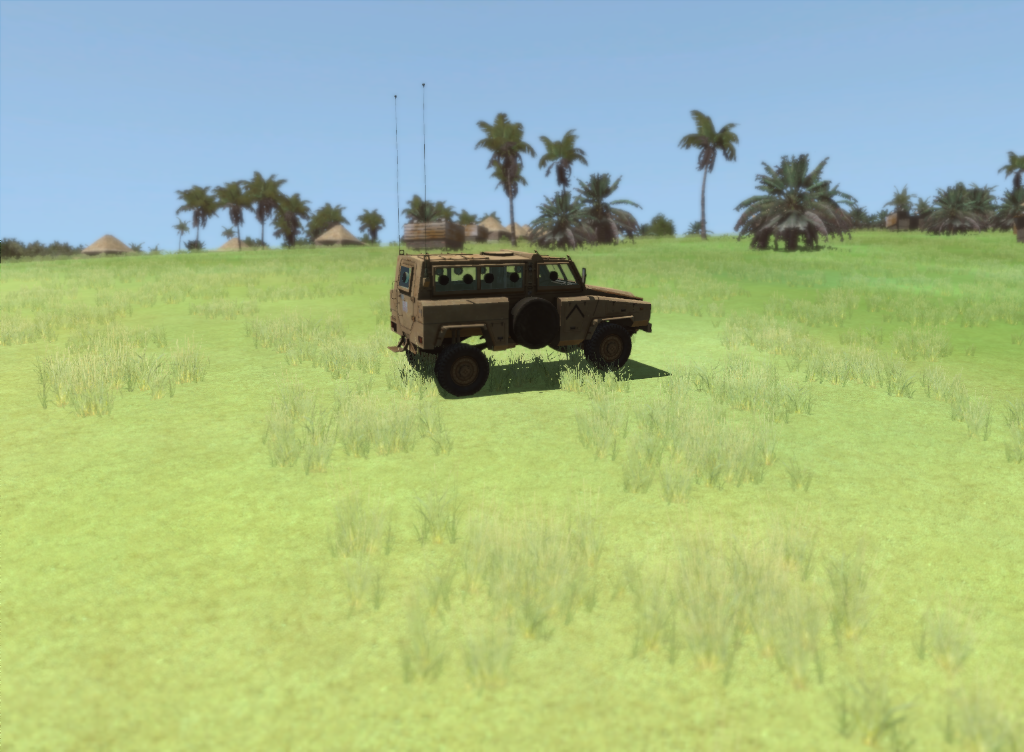
\includegraphics[height=2.4cm, width=3.4cm]{images/vbs3/realistic-lighting/light-variation/car/1.png}}
\subcaptionbox{}%
  {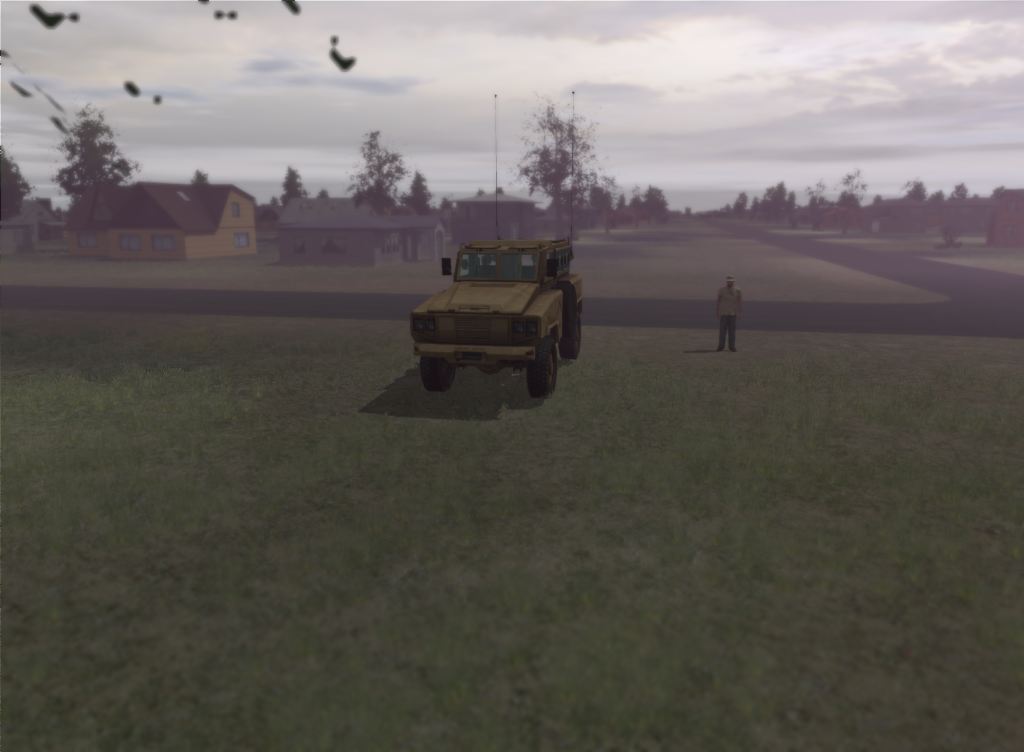
\includegraphics[height=2.4cm, width=3.4cm]{images/vbs3/realistic-lighting/light-variation/car/2.png}}
\subcaptionbox{}%
  {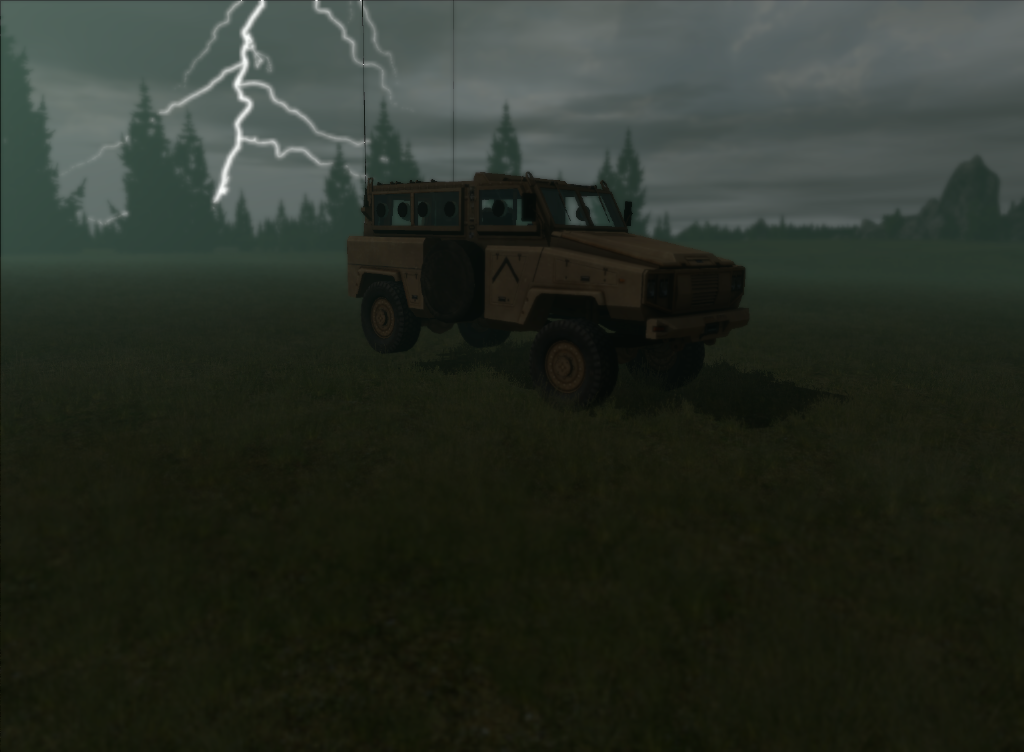
\includegraphics[height=2.4cm, width=3.4cm]{images/vbs3/realistic-lighting/light-variation/car/3.png}}
\subcaptionbox{}%
  {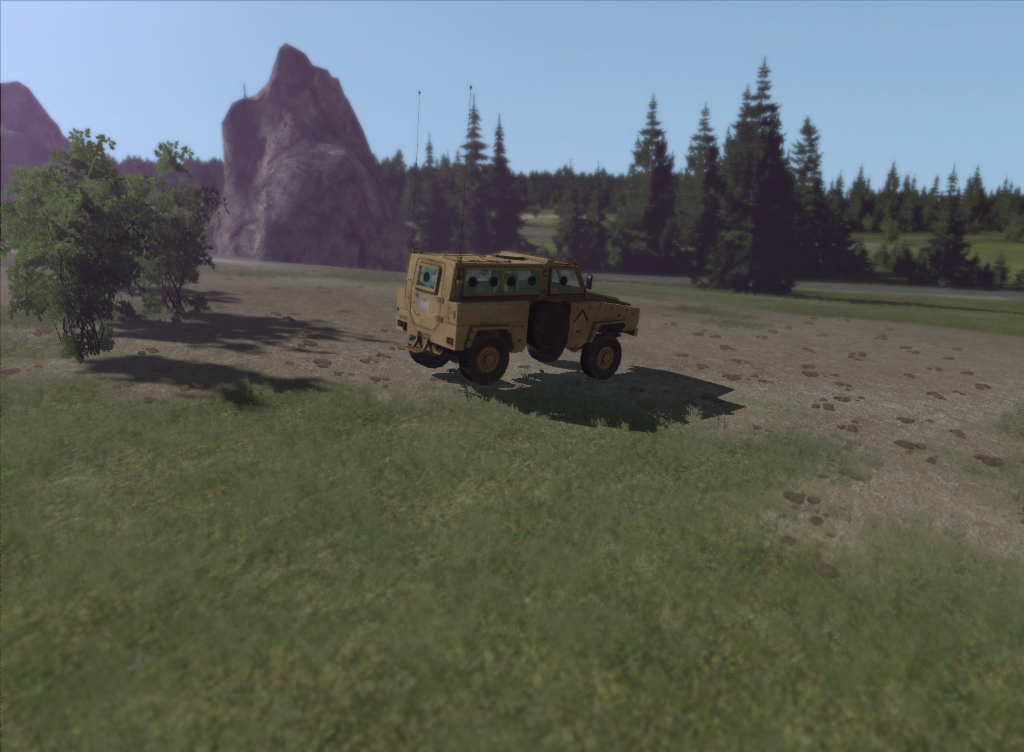
\includegraphics[height=2.4cm, width=3.4cm]{images/vbs3/realistic-lighting/light-variation/car/4.png}}
\caption{Examples of randomized lighting configurations}
\label{lighting-example}
\end{figure}

\subsection{Generated Datasets} \label{dataset-summary}
In order to evaluate how different randomization settings affects final performance, seven datasets were generated with one or more of the image randomization settings turn on or off. The settings include: \textit{crepuscular Rays, weather, time, context} and \textit{texture} randomization. If \textit{Crepuscular Rays/God Rays} was enabled, the simulation light in each image would be shifted into a random color. If \textit{Weather} was enabled the weather of the simulation was randomized for each photo. If \textit{Time} was enabled, the sun was randomly positioned somewhere in the sky. If \textit{Context} was disabled, the vehicles were positioned without any regard to how their real-world counterparts would behave, while if it was enabled the vehicles were positioned realistically. If \textit{Texture} was enabled, the texture of the vehicles was randomized in each image. These settings have been outlined in further detail in Section \ref{randomization-settings}.

All possible parameter configurations were not tested due to time constraints. For a full outline of all the generated datasets, see Table~\ref{rand-table1}. A \checkmark indicates that that randomization factor was active during the generation of that dataset, while \xmark ~indicates the setting was disabled.

Lighting was hypothesized to be the most critical factor in the generation process since it had previously been shown to have a significant effect on other tasks \cite{domainrand, goodsynthetic}. The first five datasets D1--D5 was therefore constructed to test the combined and individual effect of each light-setting. D1 tests the combined effect of all light settings, while D2 tests how completely static light effects performance. D3--D5 tests the effect of disabling of of the light parameters, in order to see their individual contribution. The last two, D6 and D7, were constructed to test if further randomization with positioning and textures could further improve accuracy.

\begin{table}[h]
\caption{Randomization configurations for the datasets}
\resizebox{\textwidth}{!}{%
  \begin{tabular}{cccccc}
  \hline
    \textbf{Dataset}  & Crepuscular Rays & Weather & Time  & Context & Texture\\
    \hline
    D1      & \checkmark     & \checkmark     & \checkmark  & \checkmark &  \xmark \\
    D2      & \xmark         & \xmark         & \xmark      & \checkmark &  \xmark \\
    D3      & \xmark         & \checkmark     & \checkmark  & \checkmark &  \xmark \\
    D4      & \checkmark     & \xmark         & \checkmark  & \checkmark &  \xmark \\
    D5      & \checkmark     & \checkmark     & \xmark      & \checkmark &  \xmark \\
    D6      & \checkmark     & \checkmark     & \checkmark  & \checkmark &  \checkmark \\
    D7      & \checkmark     & \checkmark     & \checkmark  & \xmark & \xmark \\
    \hline
  \end{tabular}}
  \label{rand-table1}
\end{table}

Since invalid image samples are filtered out after the generation process, there is not a fixed number of samples per class, and the number could vary depending on how small and likely to be obscured the vehicle models were. Similarly, some of the classes were removed if the number of samples was insufficient to sample training samples from. The exact number of data-samples per class can be seen in Table \ref{datasets}.


\begin{table}[h]
\caption{Synthetic dataset statistics}
\label{datasets}
\begin{tabular}{lSSS}
        \hline
        Dataset & \text{\# of classes} & \text{Avg. \# per class} & \text{Total}
        \\\hline        
        D1 & 2357 & 45.14806958 &    106414
        \\ 
        D2 & 2357 & 46.0767925329  &    108603
        \\ 
        D3 & 2358 & 46.0843935539  &    108667
        \\ 
        D4 & 2356 & 45.318336163  &    106770
        \\ 
        D5 & 2357 & 45.14806958  &     106414
        \\ 
        D6 & 2357 & 45.0377598642  &    106154
        \\ 
        D7 & 2342 & 48.1011955594  &    112653
        \\\hline
 \end{tabular}
\end{table}


\subsection{Summary}
The image generation process consists of: for each map and each vehicle model, randomly position the vehicle in the world, randomly position the camera around it, randomize parts of the scene, take an image and save it along with meta-information about the scene. 

The generation process had five parameters that could be adjusted in order to change how the images were randomized. To test the effect of the different parameters, seven different parameter configurations were selected and used to generate datasets containing over 106,000 images.

\section{Meta Training}\label{meta-section}
After a synthetic dataset with the desired properties have been generated, the data was used to train a model using \gls{MAML}~\cite{maml} (see Section \ref{maml}). After the training was finished, the model's performance was evaluated on a set of real-world tasks. This section will outline the setup and methods that were used when training and evaluating the models.

\subsection{Task Generation}\label{task-generation}
One of the most fundamental aspects of methods like \gls{MAML}~\cite{maml} is sampling from a task distribution $p(T)$. A task is sampled from a dataset by first uniformly sampling a set of $N$ classes without replacement from the list of classes in the dataset. A set of training and validation samples are then sampled from the selected classes (see Section \ref{maml} and Algorithm \ref{alg:maml}) without replacement and any overlap.

\subsection{Problem Settings}
For this thesis, three problem settings were explored: 5-way 1-shot, 5-way 5-shot and 5-way 10-shot classification. The 1-shot and 5+shot task utilized regular \gls{MAML} during meta-training. The 10-shot task used \gls{FOMAML} instead of regular \gls{MAML}, since regular \gls{MAML} consumed to much video-memory for that many samples. For all of tasks, a meta-batch size of four and five gradient update steps was used. Ten validation images per class were used for each task. These settings were chosen primarily as a result of hardware limitations since increasing the meta-batch size exhausted the GPU's memory resources, while setting a lower meta-batch size and lowering the number of update steps slowed down training significantly.

\subsection{Image Pre-Processing}
For each image in each task, a square area around the object of interest was cropped. The crop was always performed such that the entire object is contained within the selected region, but is randomly readjusted as not to have the object be in the center. The cropped region was then re-sized to a resolution of 128x128 using bilinear interpolation. The resulting resolution was significantly larger compared to other common meta-learning tasks like Omniglot~\cite{omniglot} or miniImageNet~\cite{matching}. This size was chosen in order to preserve as much detail of the object as possible, in order to allow the model to distinguish between superficially similar objects like different kinds of tanks or different kinds of cars.

\subsection{Image Augmentation}
Data augmentation methods were also applied to all images during the meta-learning phase. These methods were chosen because they have been previously shown to be useful when training with synthetic data ~\cite{structureddomainrandomization}. These methods include:

\begin{itemize}
    \item \textbf{Random Flipping}: Images were flipped horizontally with a 50\% chance.
    \item \textbf{Random Contrast}: The contrast of the images was randomized between 60\% and 115\% of the original contrast.
    \item \textbf{Random Saturation}: The saturation of the images was randomized between 60\% and 150\% of the original image saturation.
\end{itemize}

\subsection{Network Architecture \& Hyperparameters}
The network architecture used in this thesis was the same architecture utilized by ~\textcite{maml} in their experiments with Convolutional Neural Networks. The network consisted of five convolutional layers with 32 convolutional filters with a receptive field size of $3\times3$ and with stride 1. Each convolutional layer used \gls{RELU} activation and was followed by a $2\times2$ max-pooling layer. Batch normalization was also applied between the convolutional operation and the \gls{RELU} activation in each convolutional layer. Lastly, a single, fully connected layer with softmax activation was used to output the final prediction vector.

During meta training the inner learning rate $\alpha$ was set to 0.01. The outer update is performed using Adam with a learning rate of $\beta =0.001$ and additional parameters being set to $\beta_1=0.9, \beta_2=0.999, \epsilon=1e-08$.

The same network was used for all the tasks, with the exception being the final fully connected layer being changed when the number of classes is changed.

\subsection{Test Data}\label{test data}
In order to evaluate the generalizing performance of the models, a small number of real-world images were collected from various sources on the internet. The collected dataset was manually labeled and consist of 42 different object classes with between 15 to 30 images per class. The classes consist of different kinds of military vehicles, such as tanks, boats, airplanes, helicopters, and motorbikes, where each class is a specific vehicle model, for example, JAS Gripen (see Figure \ref{real-images} for examples). %Most of these vehicles do not have a model counterpart in any of VBS3 Datasets. This choice of using mostly new validation classes was made to highlight this approach's ability to generalize to new classes, while also bridging the reality gap.

% Real Images
\begin{figure}[H]
\centering
\subcaptionbox{}
  {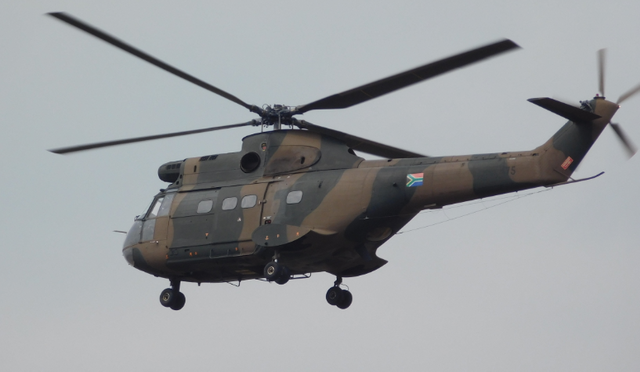
\includegraphics[height=2.4cm, width=2.4cm]{images/real-images/helicopter/1.png}}
\subcaptionbox{}%
  {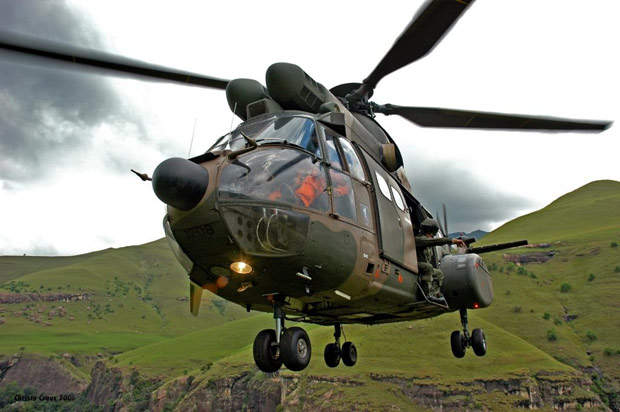
\includegraphics[height=2.4cm, width=2.4cm]{images/real-images/helicopter/2.jpg}}
\subcaptionbox{}%
  {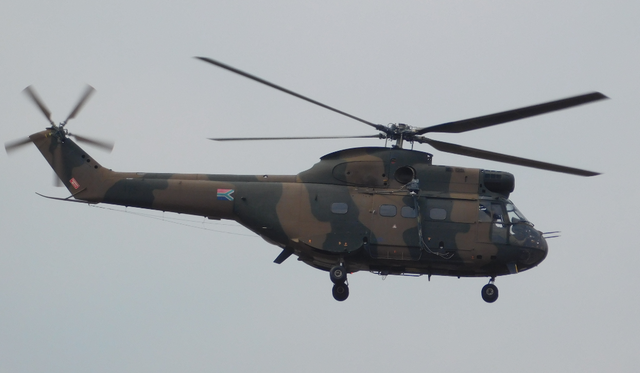
\includegraphics[height=2.4cm, width=2.4cm]{images/real-images/helicopter/3.png}}
\subcaptionbox{}
  {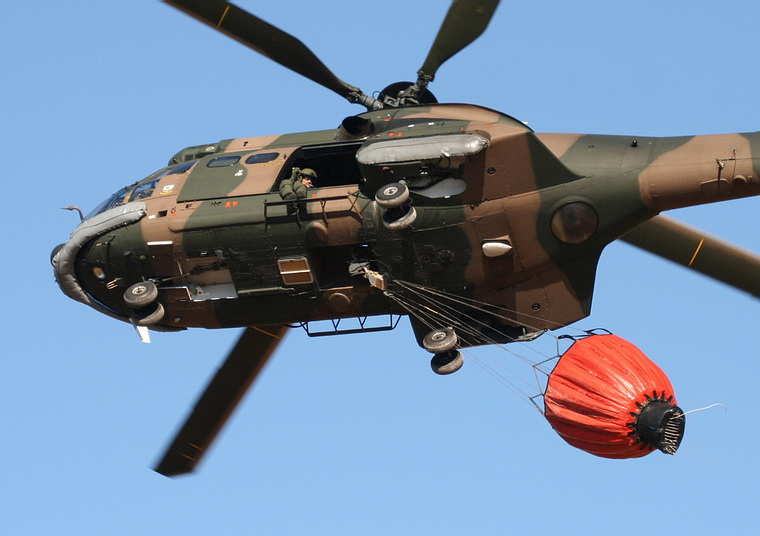
\includegraphics[height=2.4cm, width=2.4cm]{images/real-images/helicopter/4.jpg}}
\subcaptionbox{}%
  {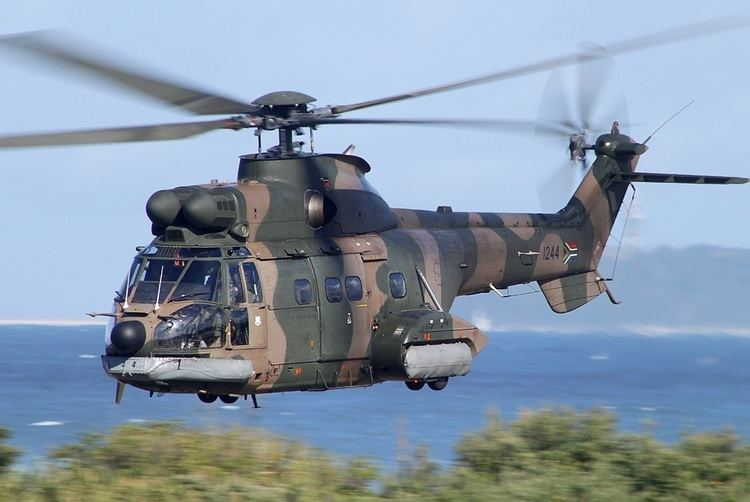
\includegraphics[height=2.4cm, width=2.4cm]{images/real-images/helicopter/5.jpeg}}

\subcaptionbox{}
  {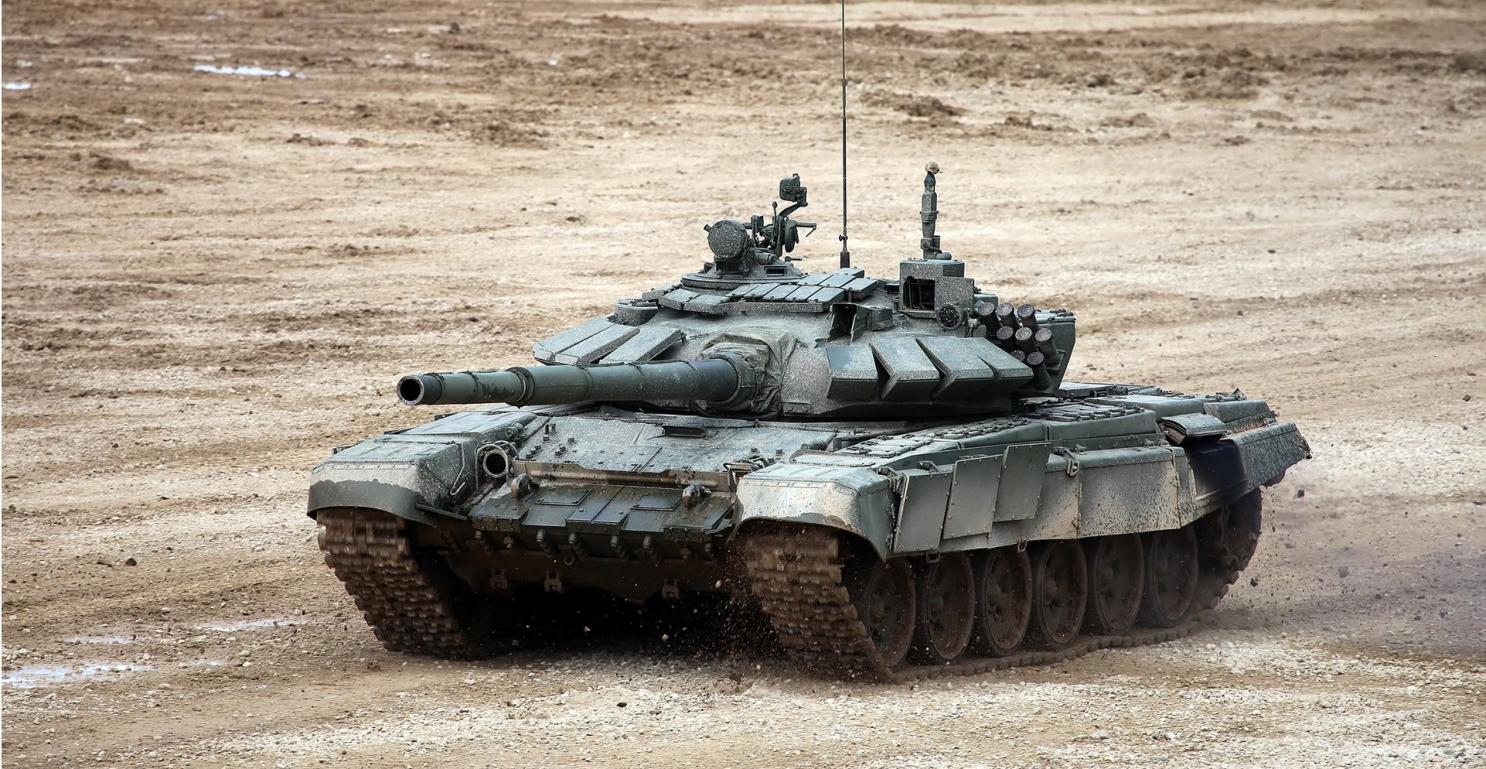
\includegraphics[height=2.4cm, width=2.4cm]{images/real-images/tank/1.jpg}}
\subcaptionbox{}%
  {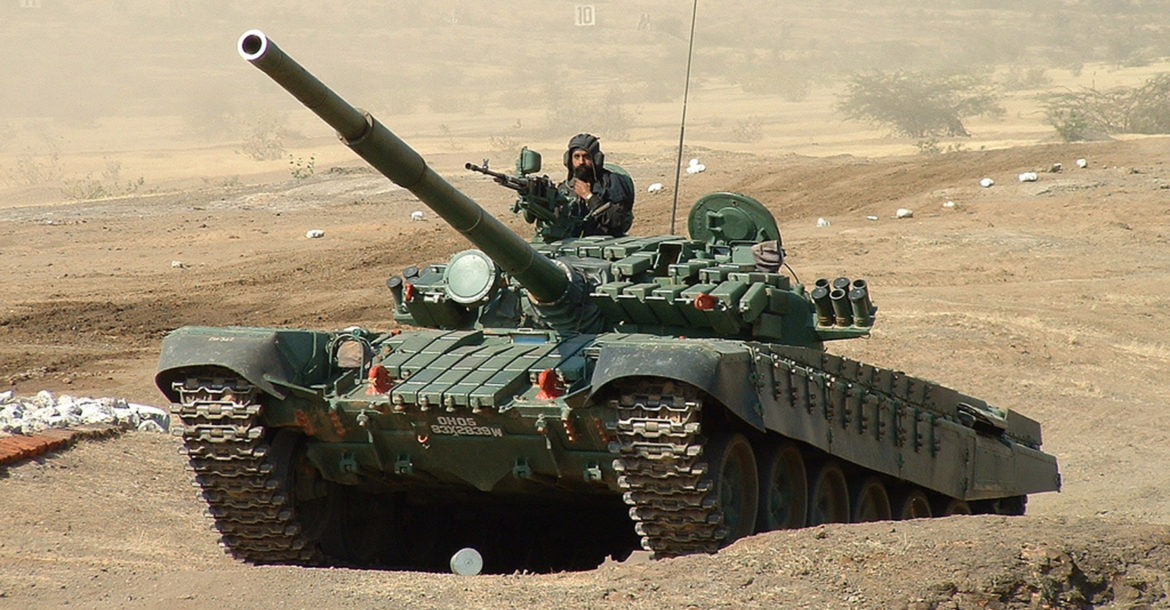
\includegraphics[height=2.4cm, width=2.4cm]{images/real-images/tank/2.jpg}}
\subcaptionbox{}%
  {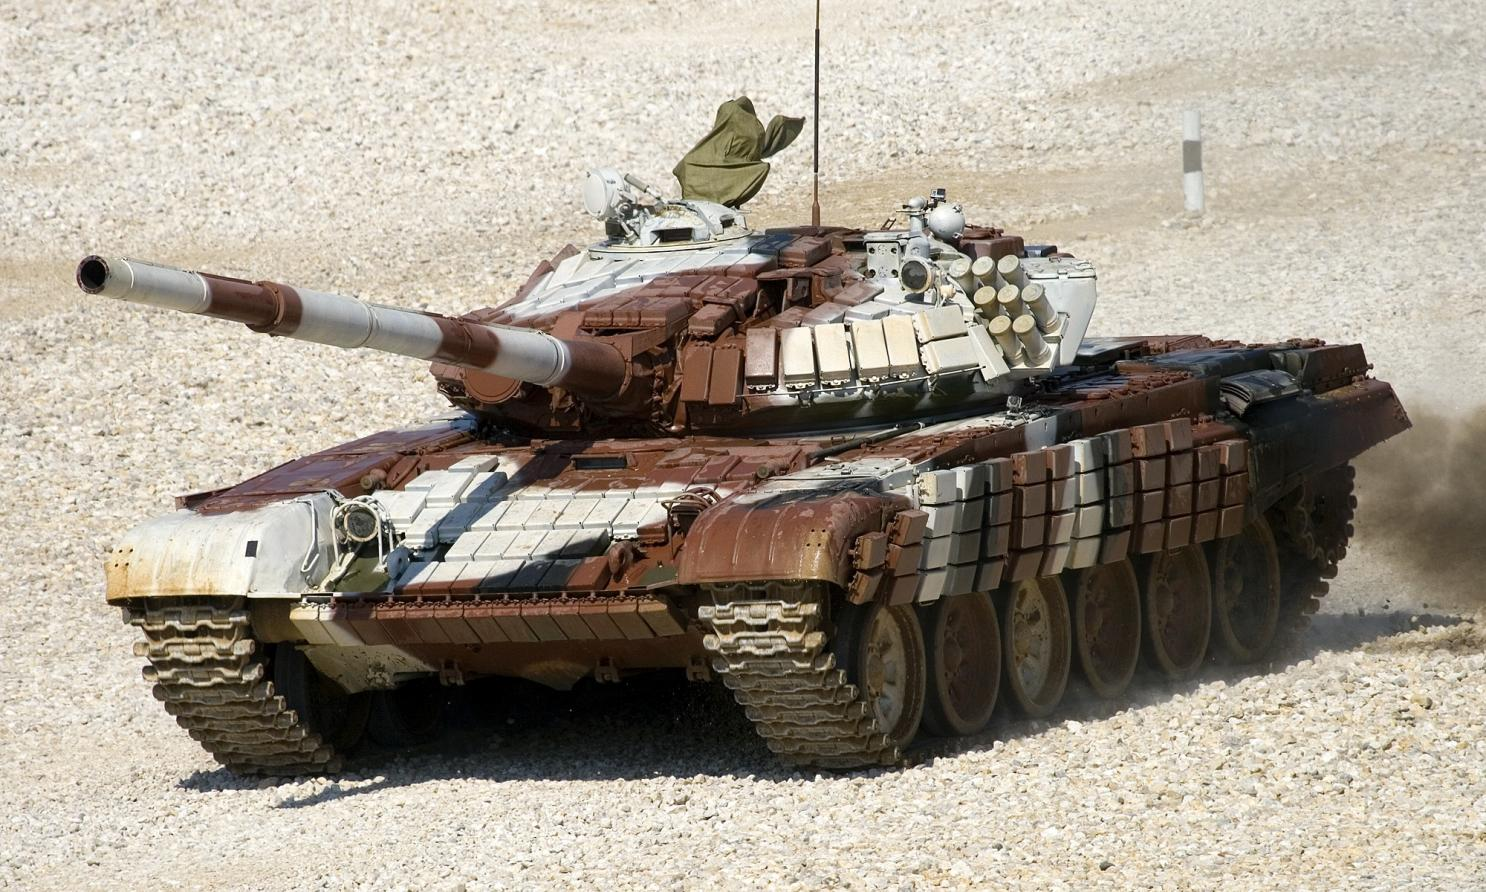
\includegraphics[height=2.4cm, width=2.4cm]{images/real-images/tank/3.jpg}}
\subcaptionbox{}
  {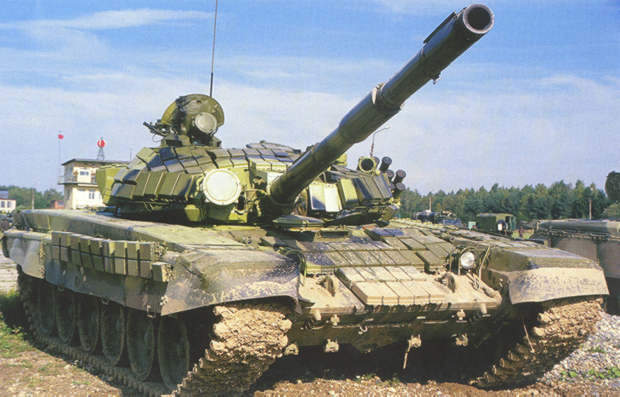
\includegraphics[height=2.4cm, width=2.4cm]{images/real-images/tank/4.jpg}}
\subcaptionbox{}%
  {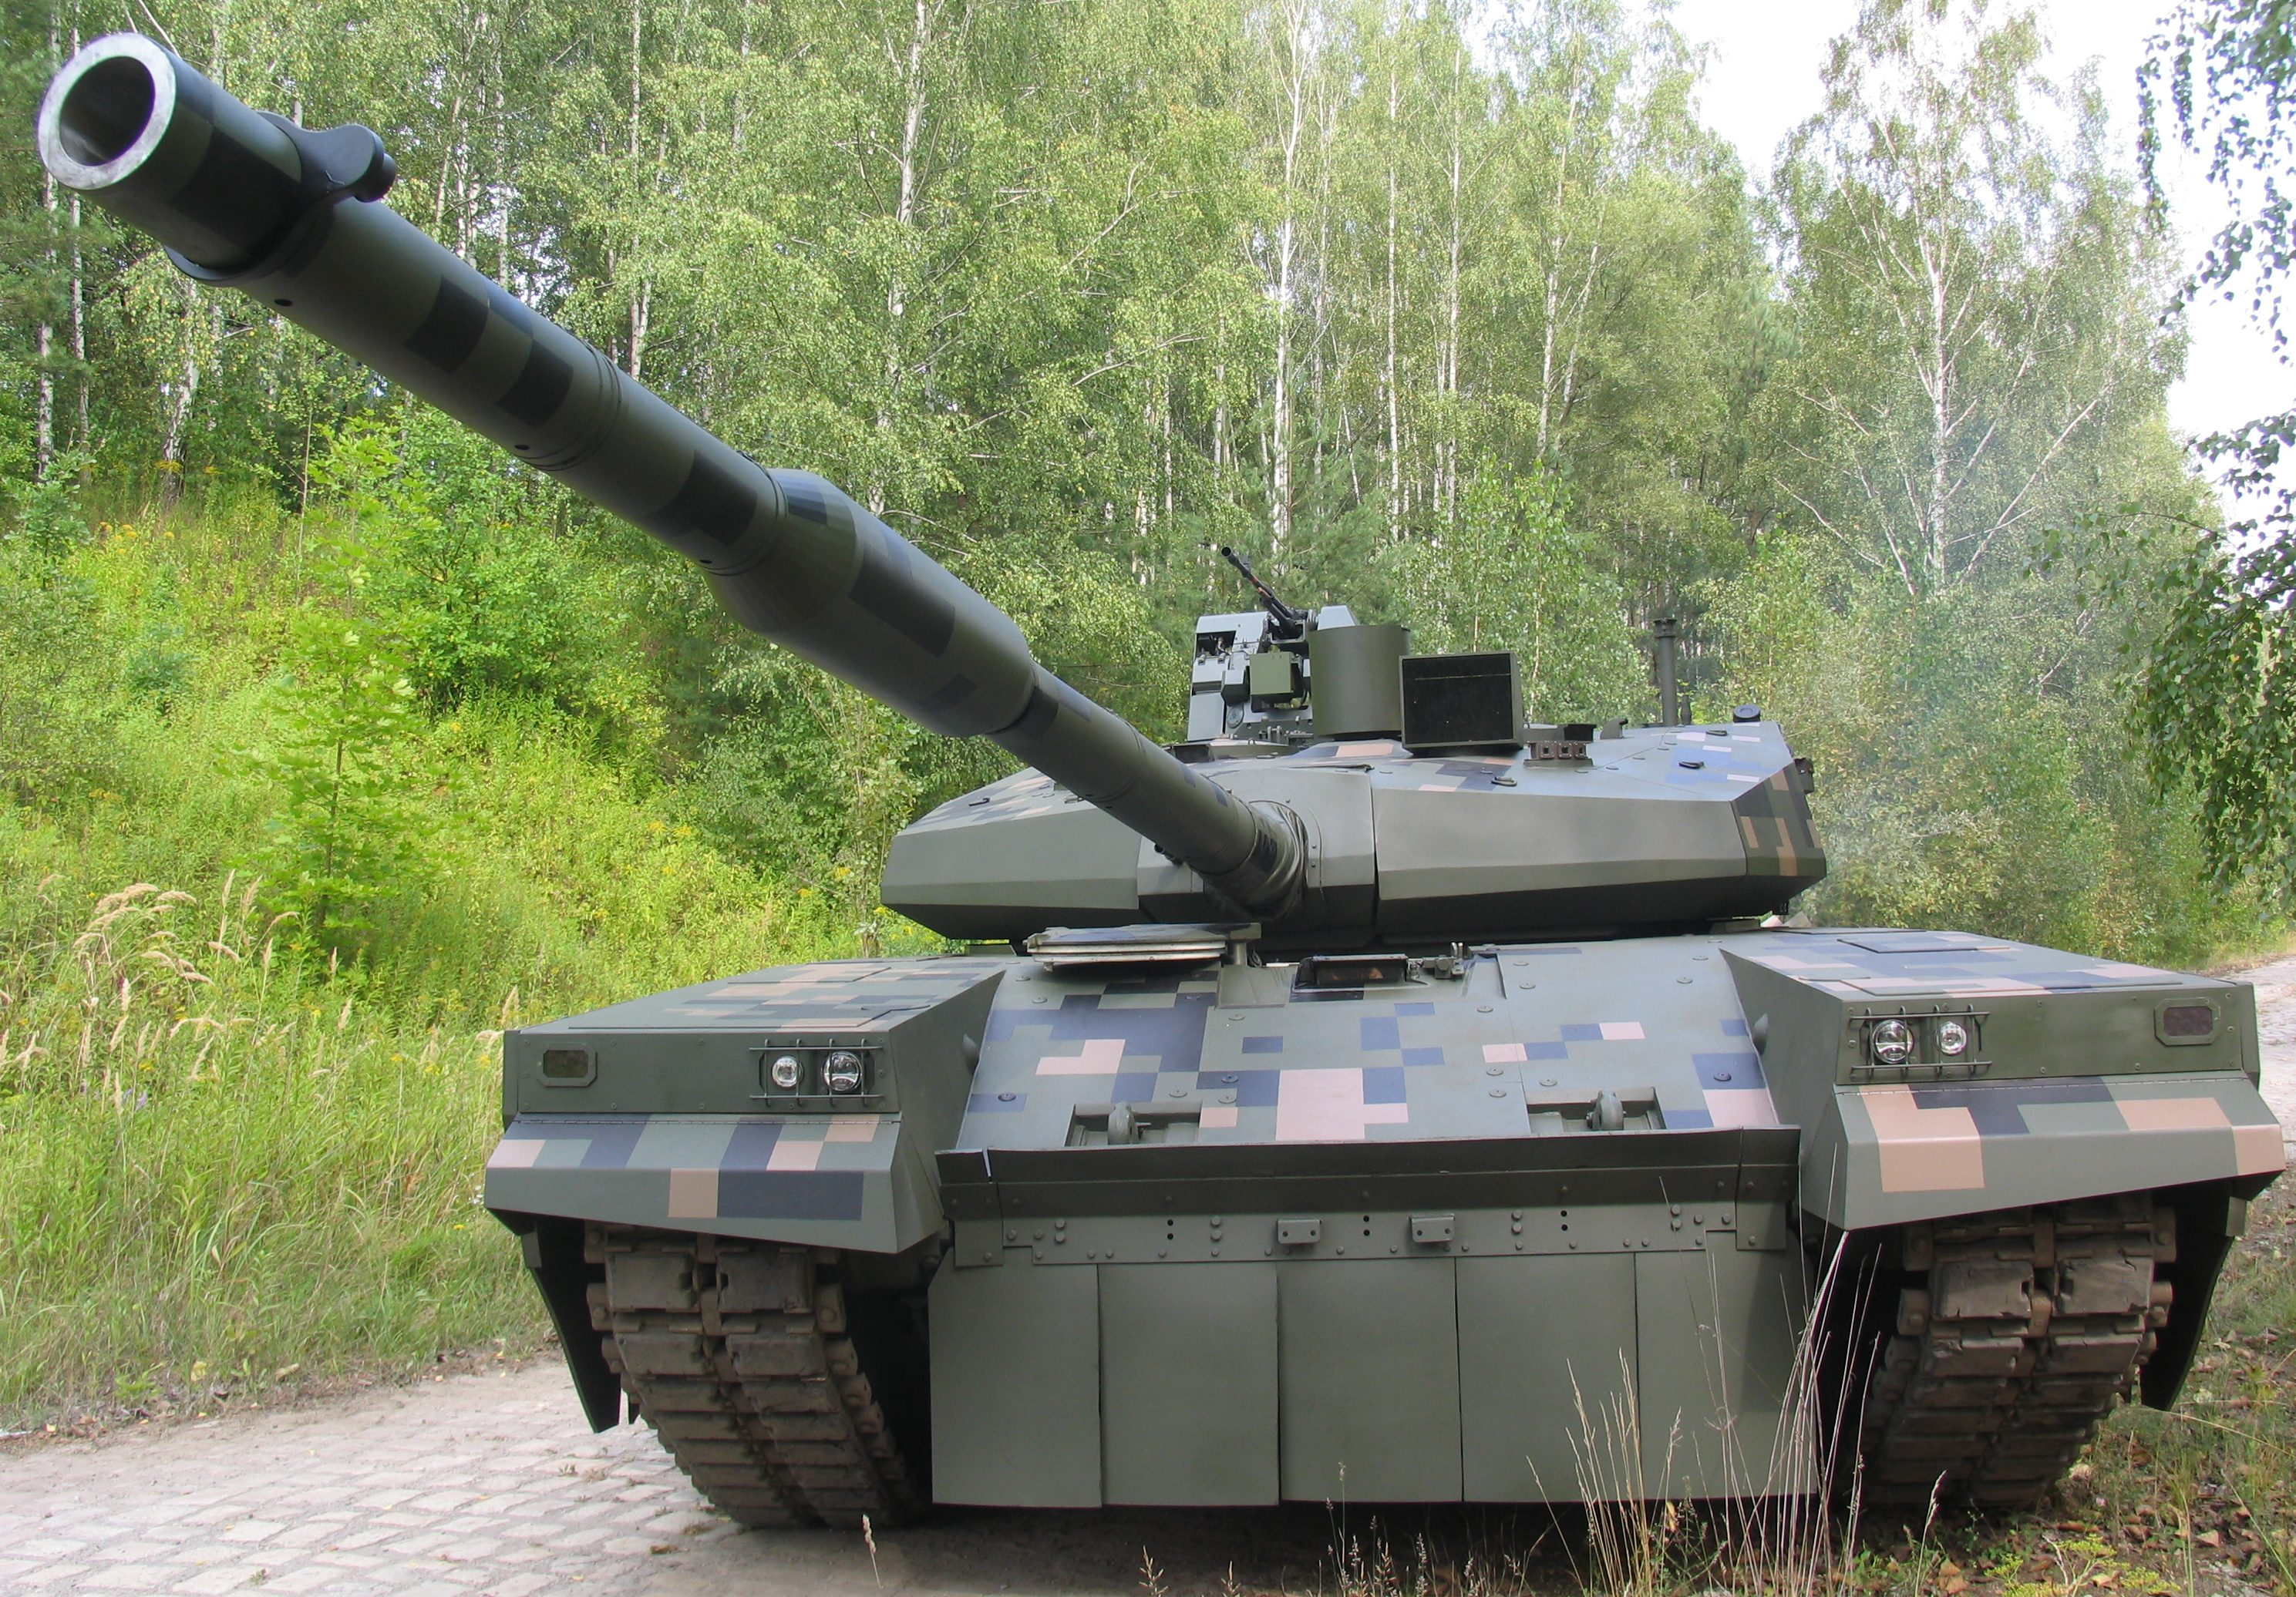
\includegraphics[height=2.4cm, width=2.4cm]{images/real-images/tank/5.jpg}}

\subcaptionbox{}
  {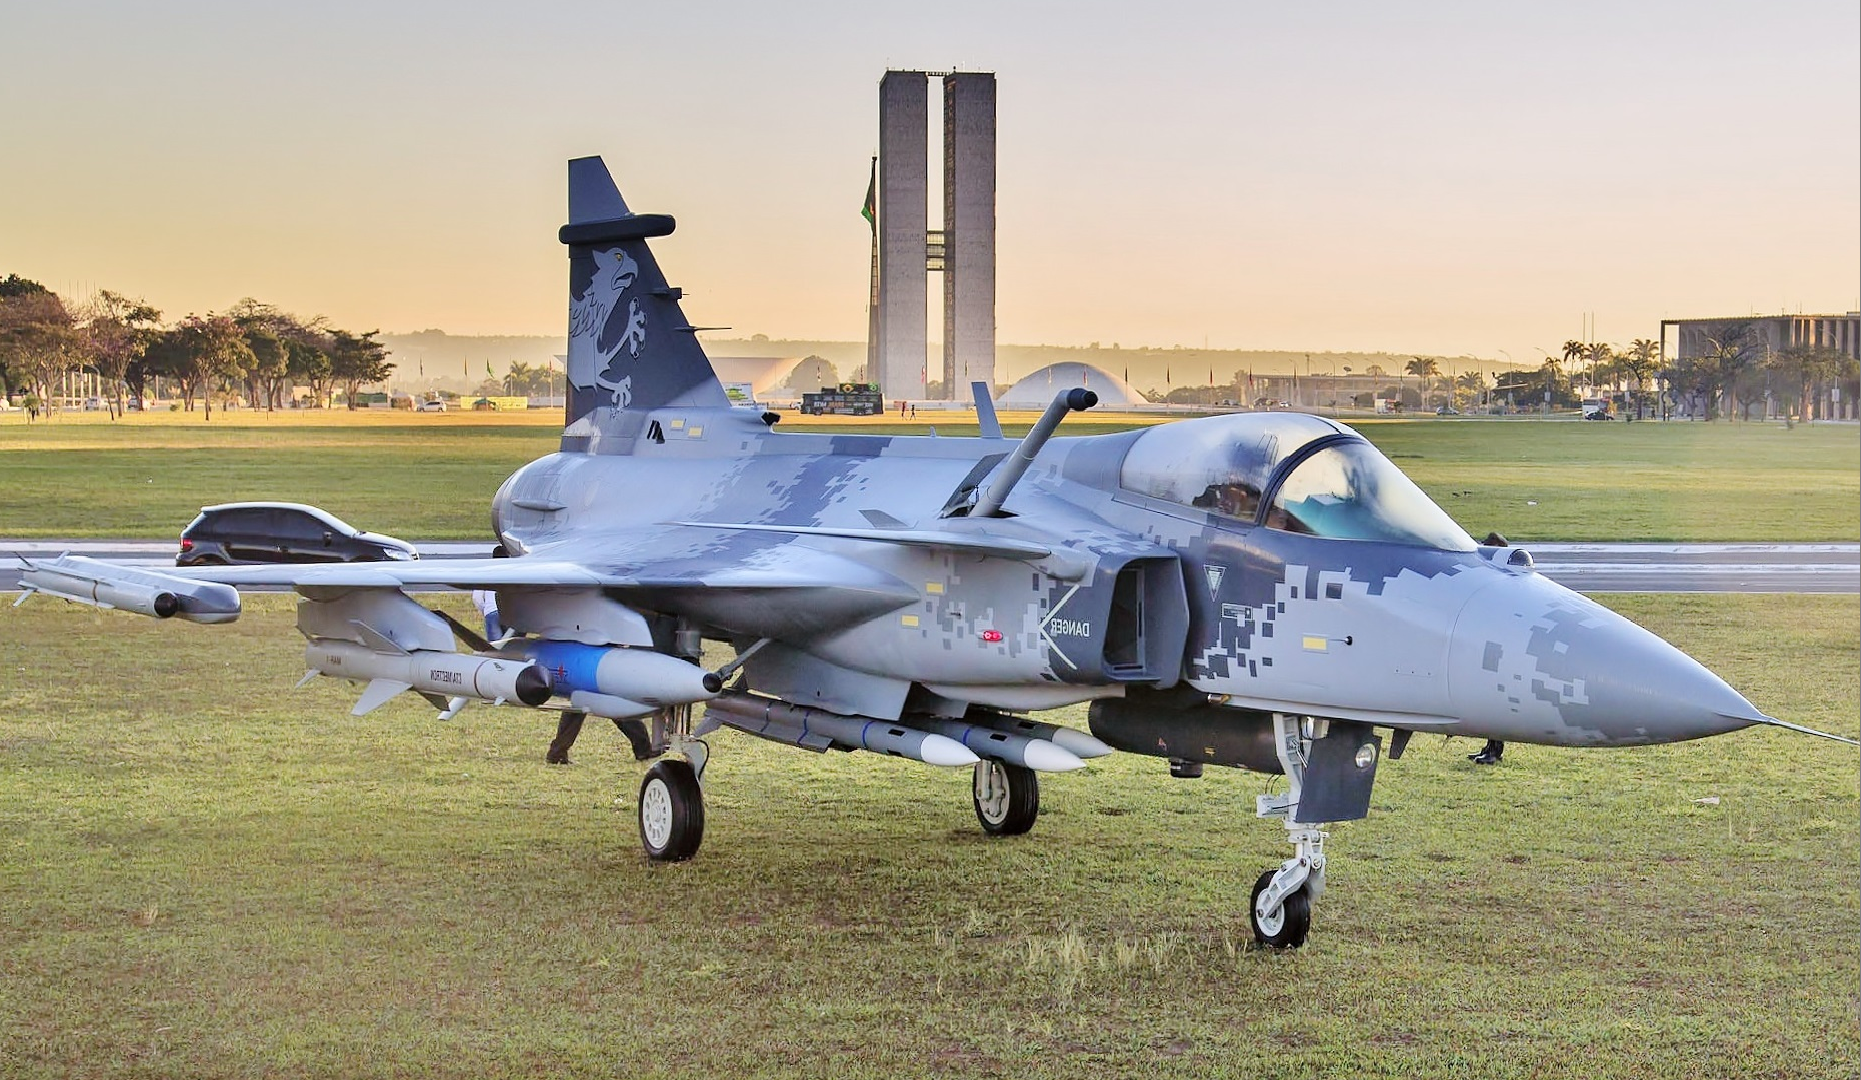
\includegraphics[height=2.4cm, width=2.4cm]{images/real-images/plane/1.png}}
\subcaptionbox{}%
  {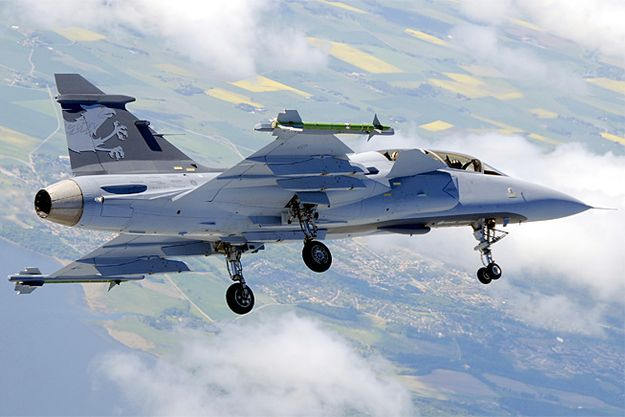
\includegraphics[height=2.4cm, width=2.4cm]{images/real-images/plane/2.jpg}}
\subcaptionbox{}%
  {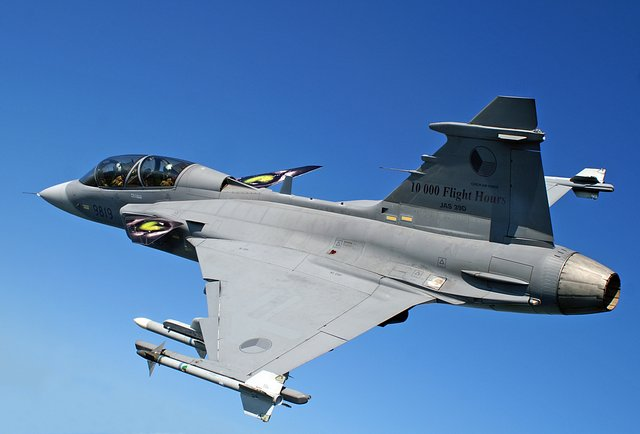
\includegraphics[height=2.4cm, width=2.4cm]{images/real-images/plane/3.jpg}}
\subcaptionbox{}
  {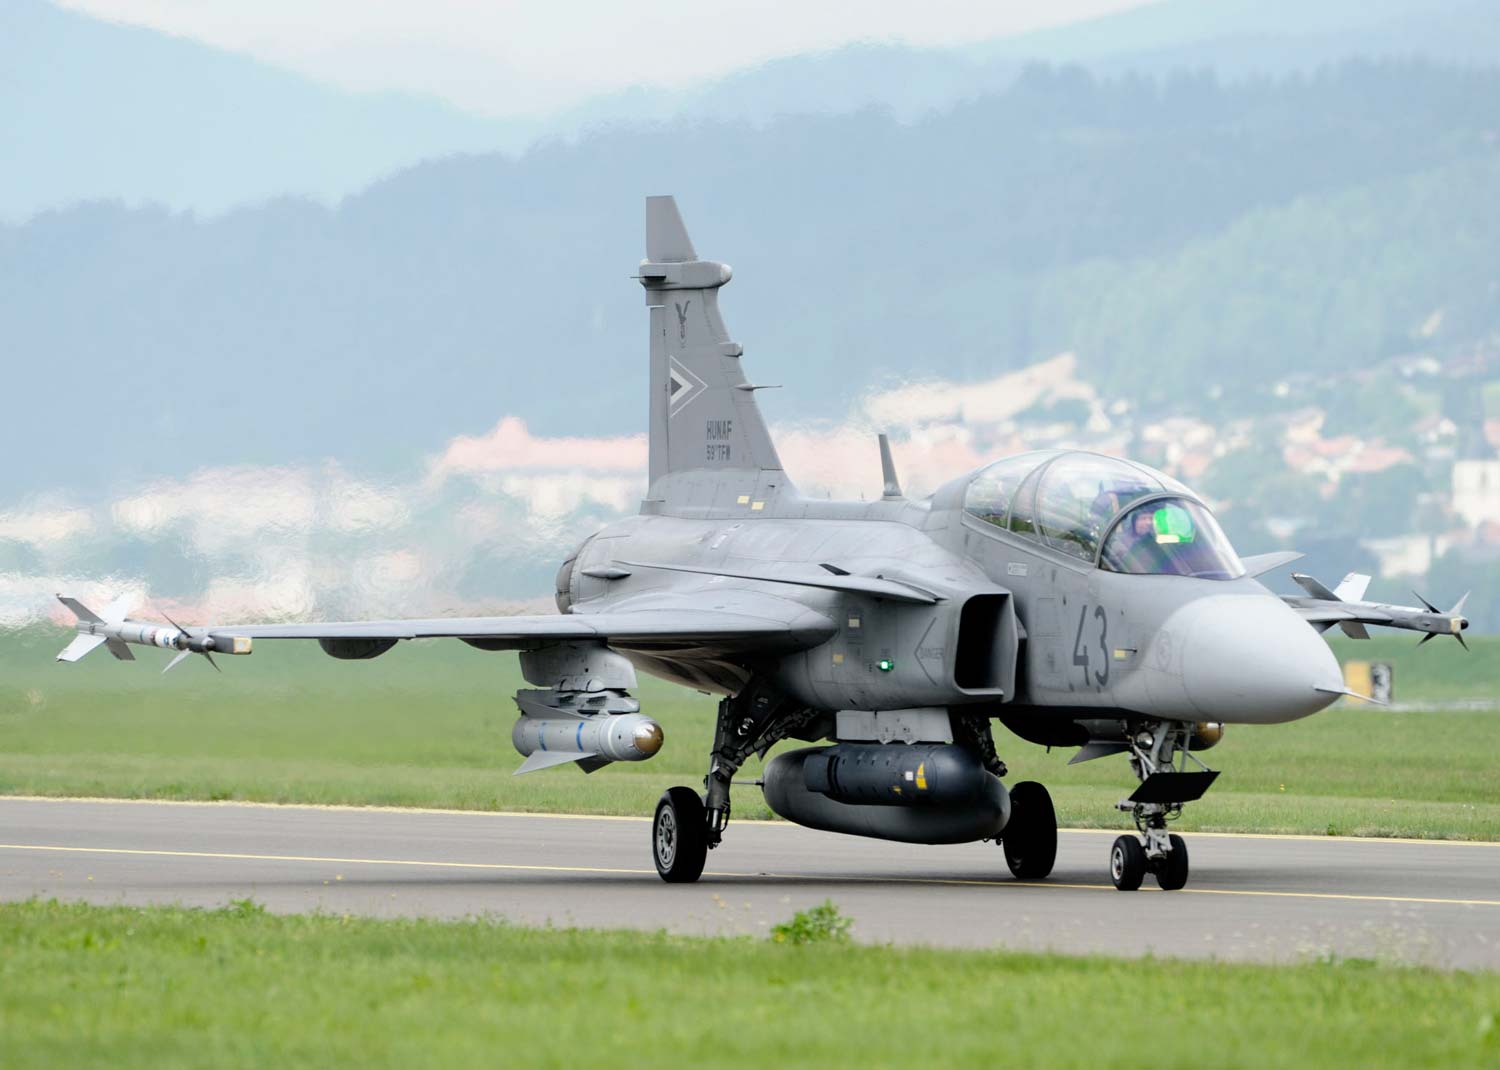
\includegraphics[height=2.4cm, width=2.4cm]{images/real-images/plane/4.jpg}}
\subcaptionbox{}%
  {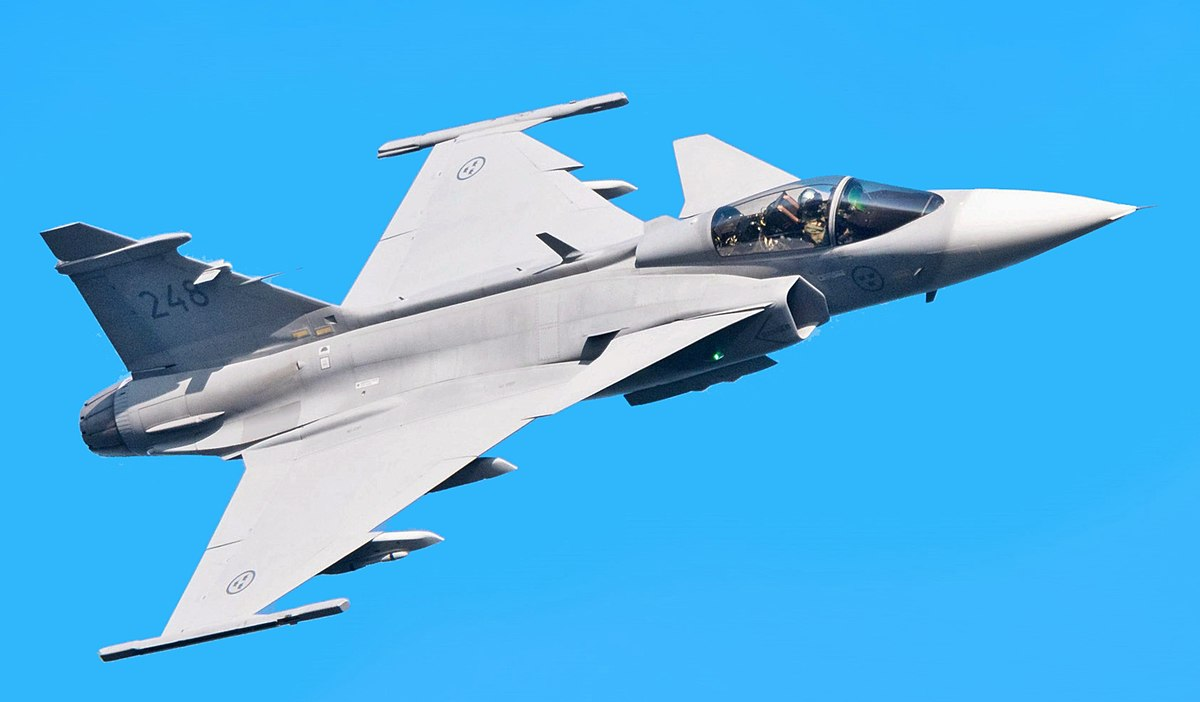
\includegraphics[height=2.4cm, width=2.4cm]{images/real-images/plane/5.jpg}}

\subcaptionbox{}
  {\includegraphics[height=2.4cm, width=2.4cm]{images/real-images/water/1.jpg}}
\subcaptionbox{}%
  {\includegraphics[height=2.4cm, width=2.4cm]{images/real-images/water/2.jpg}}
\subcaptionbox{}%
  {\includegraphics[height=2.4cm, width=2.4cm]{images/real-images/water/3.jpg}}
\subcaptionbox{}
  {\includegraphics[height=2.4cm, width=2.4cm]{images/real-images/water/4.jpg}}
\subcaptionbox{}%
  {\includegraphics[height=2.4cm, width=2.4cm]{images/real-images/water/5.jpg}}
\caption{Examples of real world images}
\label{real-images}
\end{figure}


\subsection{Performance Evaluation}
After a model had been trained using \gls{MAML} on a synthetically generated dataset, the model's ability to adapt to a real-world task was evaluated. From the dataset described in Section \ref{test data}, tasks were sampled in the same fashion as outlined in Section \ref{task-generation}. The models were given the same number of samples for each class as was defined by the few-shot classification task it was meta-trained on. Then the model was updated using batch gradient descent with a learning rate of 0.01, same as during meta-training. 

Five-thousand tasks were randomly sampled for evaluation, and the models are trained with ten gradient steps for each task. The mean of the model's accuracy after the final update-step, over five-thousand tasks, was then reported as the final accuracy.

\subsection{Baselines}
For this thesis, two baselines were chosen: First, a baseline model named BL1. This baseline involved training the same network used in all other settings, using only the meta-test data, without doing the meta-trained. This baseline was used to give an indication both how difficult the final tasks were to perform and how well the \gls{MAML} algorithm improves performance.

Secondly, a second baseline model was trained using a hand-labeled real-world dataset, collected from Bing and Google Image Search. This baseline was named BL2 and was used to highlight how the synthetic performs in comparison to models trained on real-world data. Its training set consists of 61 different vehicles, with each class consisting of between 80 to 350 RGB images. In total, the number of images is 9954.

\change{Moved to discussion}

\subsection{Summary}
The experiments consisted of training a six-layer \gls{CNN} using \gls{MAML} for each of the seven synthetic datasets (see Table \ref{datasets}). Also, two baselines were trained, one where no pre-training was used (BL1), and one that was trained using \gls{MAML} on a real-world dataset (BL2). Their performance was evaluated by sampling five-thousand tasks from a real-world test dataset and having the networks adapt to each task and then calculating the average accuracy.

\section{Programming Libraries and Frameworks} \label{software}
A mix of Python 3.7+ and the \gls{SQF} scripting language was used to generate the images in VBS3. 

\gls{SQF} is a scripting language developed by Bohemia Interactive Simulations and is used for scenario scripting within the simulation. In this thesis, it was the primary tool for controlling the simulation process, creating scenes, spawning, and iterating over objects and collection and outputting relevant vehicle information.

All other code relating to both the image generation post-processing and all the machine learning code was written in Python 3.7+. Python is a high-level scripting language with a large user-base within the machine learning community, making it the obvious choice for most things machine learning. 

Google's Tensorflow~\cite{tensorflow} library was used to construct machine learning models. Tensorflow is an open source software library developed for high-performance numerical computation. It is used both within the industry and for research applications. The implementation of the meta-learning algorithm was built using Tensorflow 1.10.0 with GPU support.

Nvidia Docker was used to constructing a virtual environment where requirements already installed to run the Tensorflow program efficiently with full GPU support. Docker is a self-contained light-weight virtual machine for which a pre-defined \textit{image} with necessary software dependencies can be installed. A copy of the docker image used to run these experiments will be made available to allow the experiments in this thesis to be easily reproduced.